\documentclass[a4paper, 12pt, british]{article} % aritcle

% make the page text 17cm wide, 24cm high
\usepackage[a4paper, total={17cm, 24cm}]{geometry}

\usepackage{amsmath}    % need for subequations
\usepackage{amssymb}    % this has \therefore
\usepackage{graphicx}   % need for figures
\usepackage{verbatim}   % useful for program listings
\usepackage{color}      % use if color is used in text
\usepackage{caption}
\usepackage{subcaption}
%\usepackage{subfigure}  % use for side-by-side figures
\usepackage{hyperref}   % use for hypertext links, including those to external documents and URLs
\usepackage{tabularx}
\usepackage{float}
\usepackage{enumitem}
\usepackage[useregional]{datetime2}

% must use lualatex to use these two
%\usepackage{fontspec}
%\setmainfont{Times}

\usepackage{fancyhdr}
\pagestyle{fancy} 
\lhead[\fancyplain{}{\bfseries\thepage}]{\fancyplain{}
	{\let\uppercase\relax\rightmark}}
\rhead[\fancyplain{}{\let\uppercase\relax\leftmark}]{\fancyplain{}
	{\bfseries\thepage}}
\cfoot[\fancyplain{}{}]{\fancyplain{}{}}


\usepackage{tocstyle}
\usetocstyle{classic}
\setcounter{secnumdepth}{3}
\setcounter{tocdepth}{2}

\numberwithin{equation}{section}
\numberwithin{figure}{section}
\numberwithin{table}{section}

% paragraph indent
\setlength{\parindent}{2em}
\setlength{\parindent}{0pt}
% paragraph spacing
\setlength{\parskip}{0.5em}

\title{CIVE3415: Water Engineering III\\ \quad \\Steady Open Channel Hydraulics}
\author{Dr Andrew Sleigh\\School of Civil Engineering\\University of Leeds}
\date{September 2019 \\ \quad \\{\scriptsize This version was created on:\\ \DTMnow}}


\begin{document}

\maketitle

\tableofcontents


\newpage 
\section{Basic Equations of Open Channel Hydraulics}
\subsection{Definition and differences between pipe flow and open channel flow}

The flow of water in a conduit may be either open channel flow or pipe flow. The two kinds of flow are similar in many ways but differ in one important respect. Open-channel flow must have a free surface, whereas pipe flow has none. A free surface is subject to atmospheric pressure. Pipe flow exerts no direct atmospheric flow but hydraulic pressure only.


\begin{figure}[H]
	\centering
	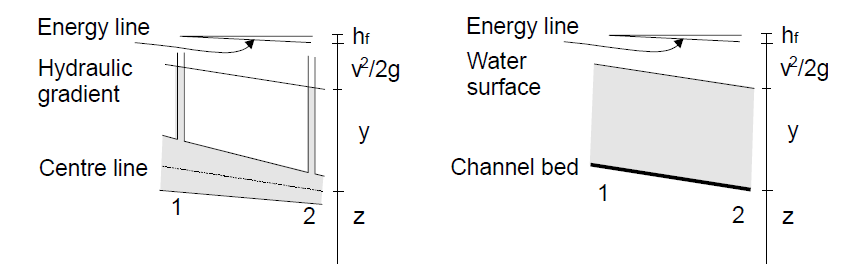
\includegraphics[scale=0.6]{./images/fig_11.png}
	\caption{Figure of pipe and open channel flow}
	\label{fig:111}
\end{figure}


The two kind of flow are compared in the figure above. On the left is pipe flow. Two piezometers are placed in the pipe at sections 1 and 2. The water levels in the pipes are maintained by the pressure in the pipe at elevations represented by the hydraulics grade line or hydraulic gradient. The pressure exerted by the water in each section of the pipe is shown in the tube by the height y of a column of water above the centre line of the pipe.

The total energy of the flow of the section (with reference to a datum) is the sum of the elevation z of the pipe centre line, the piezometric head y and the velocity head $V^2/2g$ , where $V$ is the mean velocity. The energy is represented in the figure by what is known as the energy grade line or the energy gradient.

The loss of energy that results when water flows from section 1 to section 2 is represented by $h_f$.

A similar diagram for open channel flow is shown to the right. This is simplified by assuming parallel flow with a uniform velocity distribution and that the slope of the channel is small. In this case the hydraulic gradient is the water surface as the depth of water corresponds to the piezometric height.

Despite the similarity between the two kinds of flow, it is much more difficult to solve problems of flow in open channels than in pipes. Flow condition in open channel are complicated by the position of the free surface which is likely to change with time and space. And also by the fact that depth of flow, the discharge, and the slopes of the channel bottom and of the free surface are all inter dependent.

Physical conditions in open-channels vary much more than in pipes - the cross-section of pipes is usually round - but for open channel it can be any shape.

Treatment of roughness also poses a greater problem in open channels than in pipes. Although there may be a great range of roughness in a pipe from polished metal to highly corroded iron, open channels may be of polished metal to natural channels with long grass and roughness that may also depend on depth of flow.

Open channel flows are found in large and small scale. For example the floe depth can be between a few cm in water treatment plants and over $10m$ in large rivers. The mean velocity of flow may range from less than $0.01 m/s$ in tranquil waters to above $50 m/s$ in high-head spillways. The range of total discharges may extend from $0.001 l/s$ in chemical plants to greater than $10000 m^3/s$ in large rivers or spillways. 

In each case the flow situation is characterised by the fact that there is a free surface whose position is NOT known beforehand - it is determined by applying momentum and continuity principles.

In general the treatment of open-channel flow is more empirical than pipe flow - but can still produce useful results.

Open channel flow is driven by gravity in most cases rather than by pressure work as in pipes.

\begin{table}[H]
	\centering
	\begin{tabularx}{\textwidth}{lXX}
		\hline
		\noalign{\vskip 2mm} 
		   & \textbf{Pipe Flow} & \textbf{Open Channel Flow}  \\ 
		\hline
		\noalign{\vskip 2mm} 
Flow driven by&	Pressure work&	Gravity (potential energy)\\
		\hline
Flow cross section &	Known, fixed&	Unknown in advance because the flow depth is unknown\\
		\hline
Characteristic flow parameters&	velocity deduced from continuity&	Flow depth deduced simultaneously from solving both continuity and momentum equations\\
		\hline
Specific boundary conditions& &		Atmospheric pressure at the free surface\\
		\hline
	\end{tabularx}
	\caption{Differences Between Pipe Flow and Open Channel FLow}
	\label{tab:11}
\end{table}


\newpage
\subsection{Types of flow}

The following classifications are made according to change in flow depth with respect to time and space.
 
\begin{figure}[H]
	\centering
	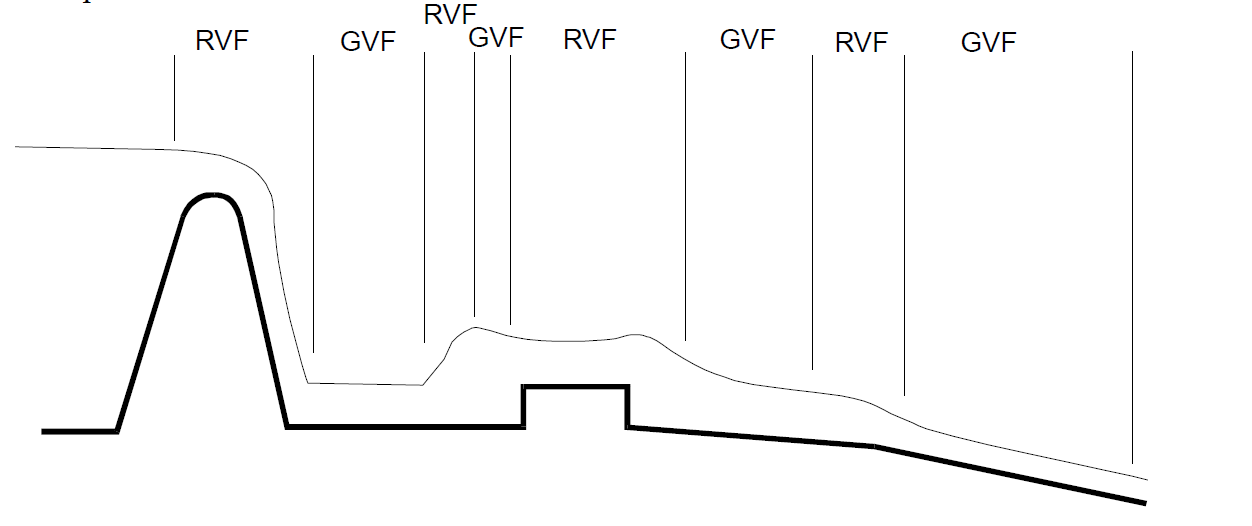
\includegraphics[scale=0.5]{./images/fig_12.png}
	\caption{Types of flow that may occur in open channels}
	\label{fig:121}
\end{figure}


\begin{itemize}
	\item \textbf{Steady and Unsteady: Time is the criterion.}\\
Flow is said to be steady if the depth of flow does not change or can be considered constant for the time interval under consideration. The flow is unsteady if depth changes with time. 

\item \textbf{Uniform Flow: Space as the criterion}.\\
Open Channel flow is said to be uniform if the depth of flow is the same at every section of the channel. A uniform flow may be steady or unsteady.

\item\textbf{Steady uniform flow}\\
Depth is constant with both time and distance.
This constitutes the fundamental type of flow in an open channel. It occurs when gravity forces are in equilibrium with resistance forces.

\item \textbf{Steady non-uniform flow.}\\
Depth varies with distance but not with time. This type of flow may be either (a) gradually varied or (b) rapidly varied. Type (a) requires the application of the energy and frictional resistance equations while type (b) requires the energy and momentum equations.

\item \textbf{Unsteady flow}\\
The depth varies with both time and space. This is the most common type of flow and requires the solution of the energy momentum and friction equations with time.
\end{itemize}

\subsection{Properties  of open channels }

\textbf{Artificial channels}\\
These are channels made by man. They include irrigation canals, navigation canals, spillways, sewers, culverts and drainage ditches. They are usually constructed in a regular cross-section shape throughout - and are thus prismatic channel (they don't widen or get narrower along the channel. In the field they are commonly constructed of concrete, steel or earth and have the surface roughness- reasonably well defined (although this may change with age - particularly grass lined channels.) Analysis of flow in such well-defined channels will give reasonably accurate results.

\textbf{Natural channels}\\
Natural channels can be very different. They are not regular nor prismatic and their materials of construction can vary widely (although they are mainly of earth this can possess many different properties.) The surface roughness will often change with time distance and even elevation. Consequently it becomes more difficult to accurately analyse and obtain satisfactory results for natural channels than is does for man-made ones. 

\subsubsection{Geometric properties necessary for analysis}
For analysis various geometric properties of the channel cross-sections are required. For artificial channels these can usually be defined using simple algebraic equations given y the depth of flow. 

\begin{figure}[H]
	\centering
	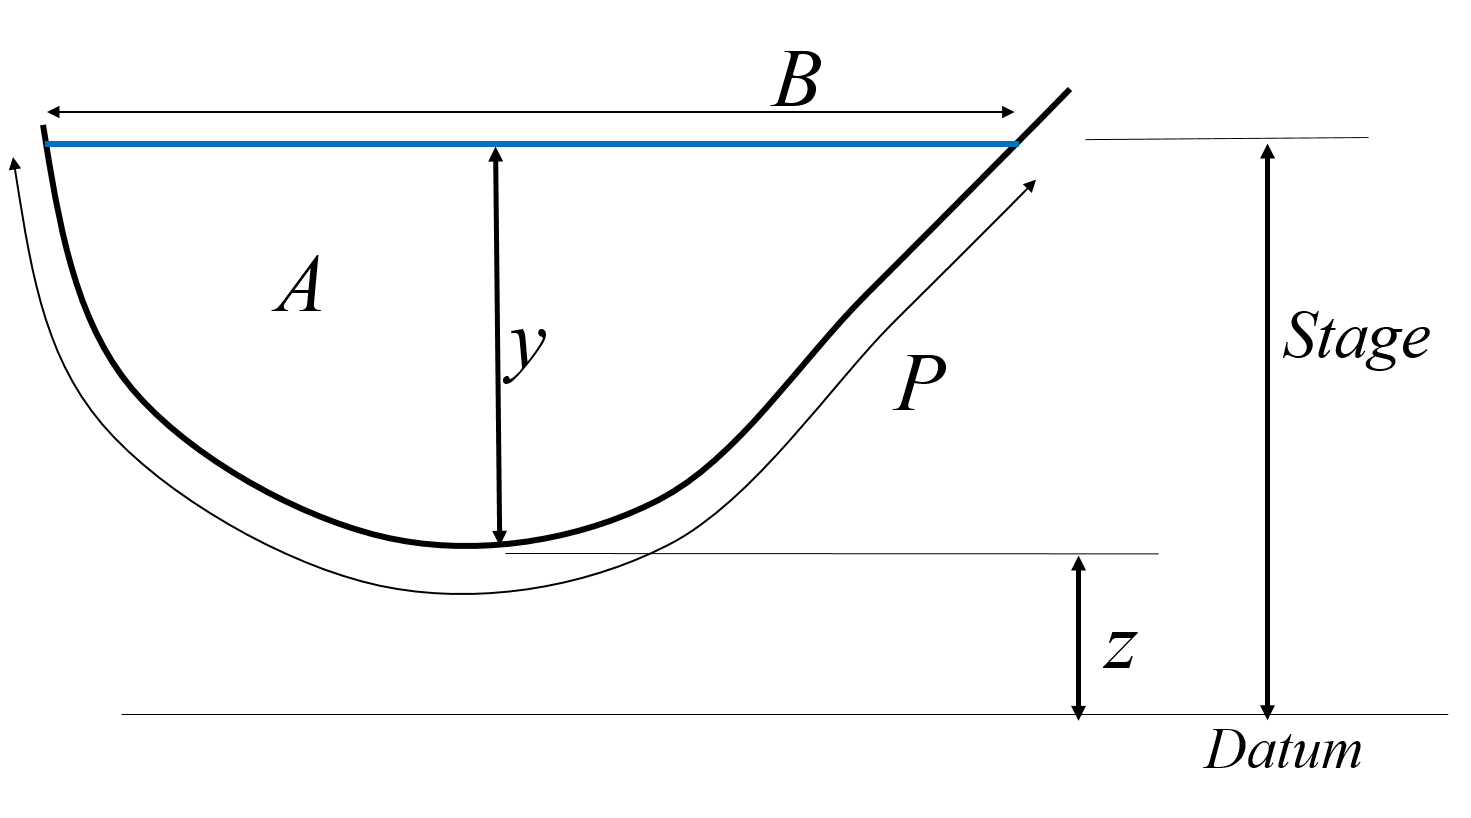
\includegraphics[width=10cm]{./images/section_general.png}
	\caption{A general section of a channel with notation}
	\label{fig:section_general_0}
\end{figure}

The commonly needed geometric properties are shown in figure \ref{fig:section_general_0} and defined as:

\begin{itemize}
	\item Depth ($y$) - the vertical distance from the lowest point of the channel section to the free surface.
\item Stage ($z$) - the vertical distance from the free surface to an arbitrary datum
\item Area ($A$) - the cross-sectional area of flow, normal to the direction of flow
\item Wetted perimeter ($P$) - the length of the wetted surface measured normal to the direction of flow.
\item Surface width ($B$) - width of the channel section at the free surface
\item Hydraulic radius ($R$) - the ratio of area to wetted perimeter (A/P)
\item Hydraulic mean depth ($D_m$) (or sometimes $\delta$) - the ratio of cross-sectional area to surface width $(A/B)$
\end{itemize}

\begin{table}[H]
	\centering
	\begin{tabularx}{\textwidth}{lccc}
		\hline
		\noalign{\vskip 2mm} 
		 & Rectangle & Trapezoid & Circle \\
		 \hline
		 \noalign{\vskip 2mm} 
		& 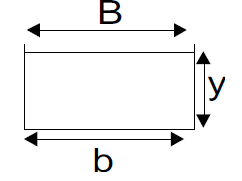
\includegraphics[scale=0.5]{./images/fig_131a.png}&  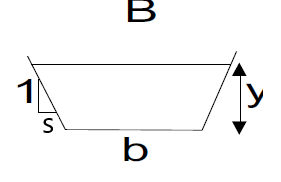
\includegraphics[scale=0.5]{./images/fig_131b.png}& 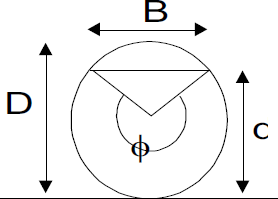
\includegraphics[scale=0.5]{./images/fig_131c.png} \\ 
						& &  & ($\phi$ in \textit{radians}) \\ 
		\hline
		\noalign{\vskip 2mm} 
		 Area, $A$ & $by$ &$(b+sy)y$ & $\frac{1}{8}(\phi - \sin \phi)D^2$ \\
		 		\hline
		 \noalign{\vskip 2mm} 
		 Wetted perimeter, $P$ &$b+2y$& $b+2y\sqrt{1+s^2}$& $\frac{1}{2}\phi D$\\
		 		\hline
		 \noalign{\vskip 2mm} 
		 Top width, $B$ &$b$ & $b+2sy$ & $(\sin(\phi/2))D$ \\
		 		\hline
		 \noalign{\vskip 2mm} 
		 Hydraulic Radius, $R = \frac{A}{P}$ & $\frac{by}{b+2y}$&$ \frac{(b+sy)y}{b+2y\sqrt{1+x^2}}$ & $\frac{1}{4}\left(1-\frac{\sin \phi}{\phi}\right)D$ \\
		 		\hline
		 \noalign{\vskip 2mm} 
		 Hydraulic mean depth, $D_m = \frac{A}{B}$ & $y$&$\frac{(b+sy)y}{b+2sy}$ & $\frac{1}{8}\left(\frac{\phi - \sin \phi}{\sin (\phi/2)}\right)D$\\
\hline
	\end{tabularx}
	\caption{Equations of Section Properties for Rectangular, Trapezoidal and Circular sections}
	\label{tab:131}
\end{table}


\subsection{Fundamental equations}

The equations which describe the flow of fluid are derived from three fundamental laws of physics:

\begin{enumerate}
	\item Conservation of matter (or mass)
\item Conservation of energy 
\item Conservation of momentum
\end{enumerate}

Although first developed for solid bodies they are equally applicable to fluids. A brief description of the concepts are given below.

\textbf{Conservation of matter}\\
This says that matter can not be created nor destroyed, but it may be converted (e.g. by a chemical process.) In fluid mechanics we do not consider chemical activity so the law reduces to one of conservation of mass.

\textbf{Conservation of energy}\\
This says that energy can not be created nor destroyed, but may be converted form one type to another (e.g. potential may be converted to kinetic energy). When engineers talk about energy "losses" they are referring to energy converted from mechanical (potential or kinetic) to some other form such as heat. A friction loss, for example, is a conversion of mechanical energy to heat. The basic equations can be obtained from the First Law of Thermodynamics but a simplified derivation will be given below.



\textbf{Conservation of momentum}\\
The law of conservation of momentum says that a moving body cannot gain or lose momentum unless acted upon by an external force. This is a statement of Newton's Second Law of Motion:

\begin{equation*}
\text{Force} = \text{rate of change of momentum}
\end{equation*}

In solid mechanics these laws may be applied to an object which is has a fixed shape and is clearly defined. In fluid mechanics the object is not clearly defined and as it may change shape constantly. To get over this we use the idea of  \textit{control volumes}. These are imaginary volumes of fluid within the body of the fluid. To derive the basic equation the above conservation laws are applied by considering the forces applied to the edges of a control volume within the fluid.

\subsubsection{The Continuity Equation (conservation of mass)}

For any control volume during the small time interval $\delta t$ the principle of conservation of mass implies that the mass of flow entering the control volume minus the mass of flow leaving the control volume equals the change of mass within.

If the flow is steady and the fluid incompressible the mass entering is equal to the mass leaving, so there is no change of mass within the control volume. 

So for the time interval $\delta t$:


 \begin{equation*}
 \text{Mass flow entering} = \text{mass flow leaving}
 \end{equation*}
 
 \begin{figure}[H]
 	\centering
 	%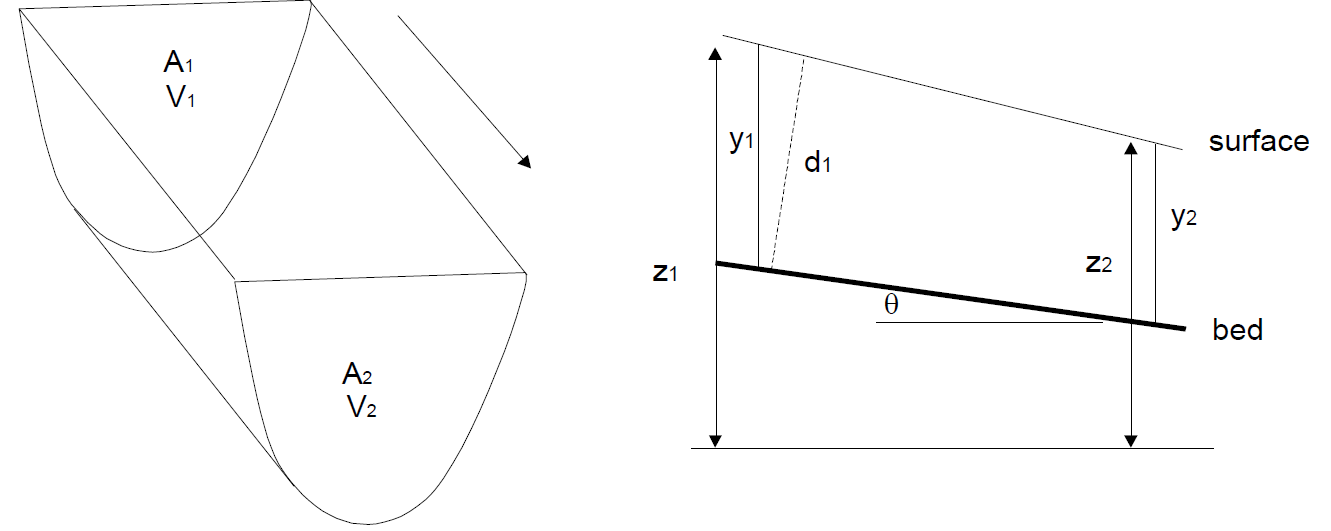
\includegraphics[scale=0.45]{./images/fig_141.png}
 	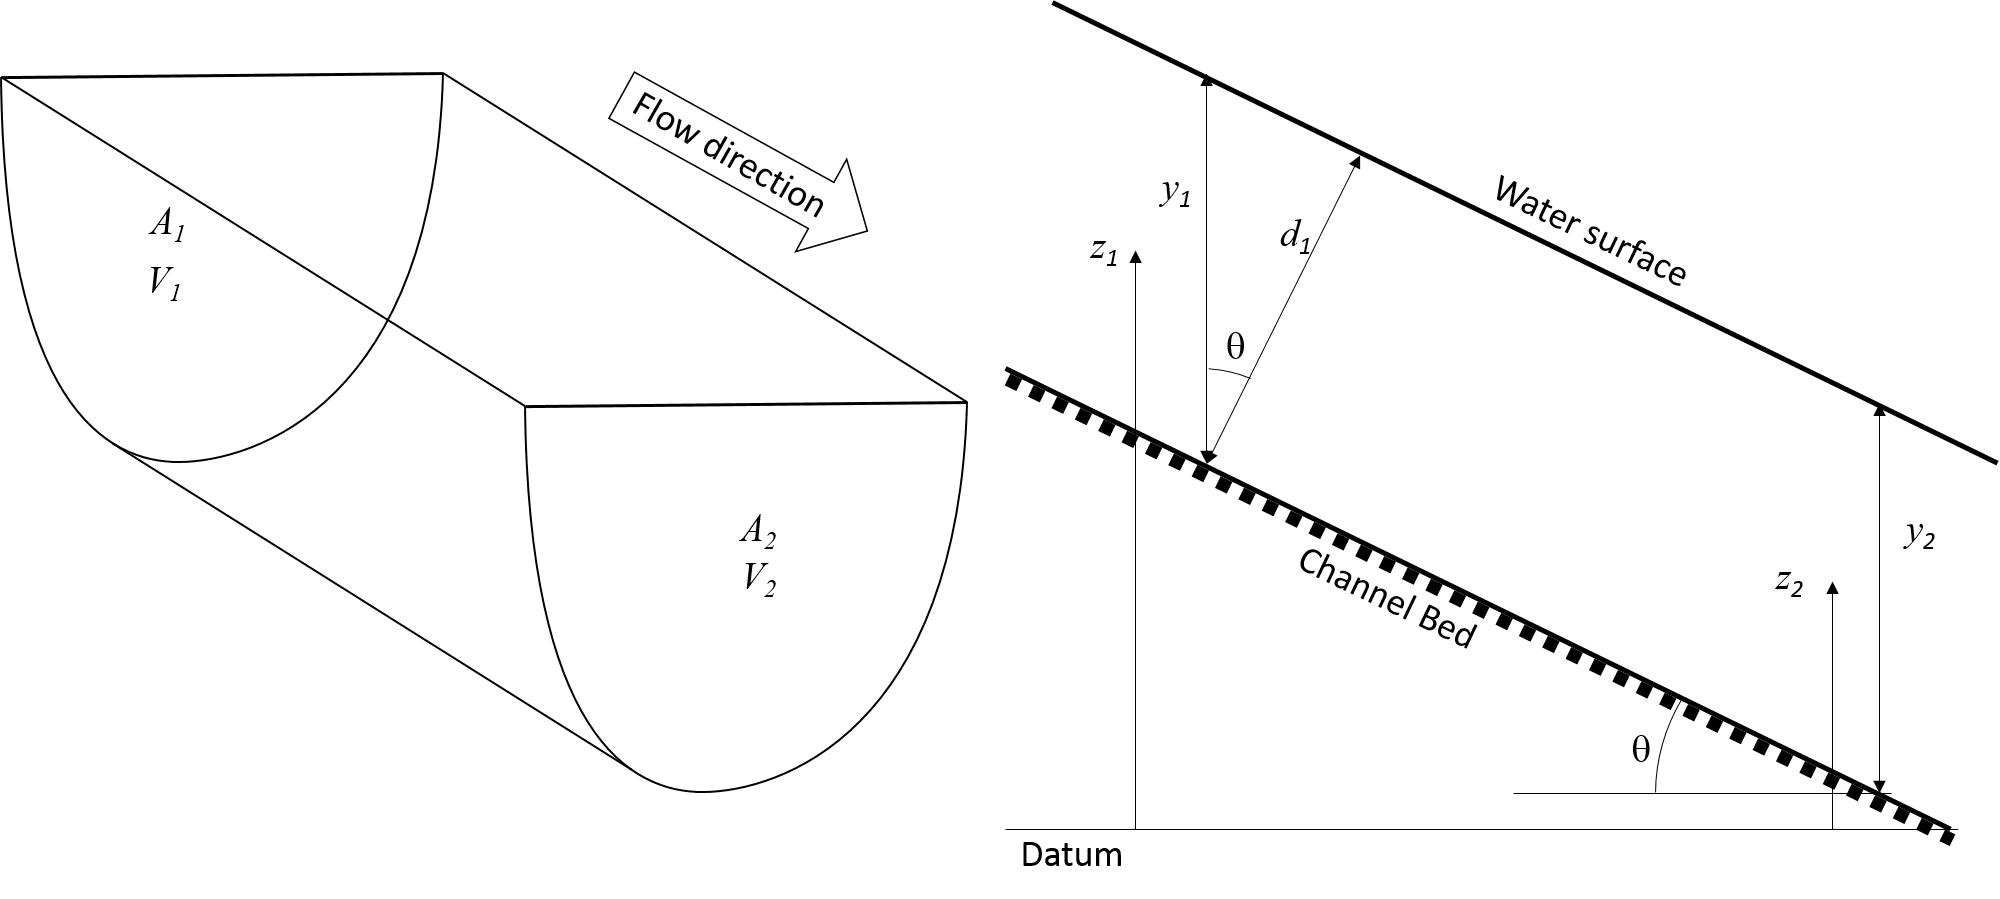
\includegraphics[scale=0.45]{./images/channel_cv_2018.png}
 	\caption{A small length of channel as a control volume}
 	\label{fig:141}
 \end{figure}


Considering the control volume above which is a short length of open channel of arbitrary cross-section then, if $\rho$ is the fluid density and $Q$ is the volume flow rate then
mass flow rate is $\rho Q$ and the continuity equation for steady incompressible flow can be written

 \begin{equation}
\rho Q_\text{entering} = \rho Q_\text{leaving}
\end{equation} 

As, $Q$, the volume flow rate is the product of the area and the mean velocity then at the upstream face (face 1) where the mean velocity is $V_1$ and the cross-sectional area is $A_1$ then:
 
Similarly at the downstream face, face 2, where mean velocity is $V_2$ and the cross-sectional area is $A_2$ then:
 
 \begin{equation}
 Q_\text{leaving} = V_2 A_2
 \end{equation}

Therefore the continuity equation can be written as

  \begin{equation}
V_1 A_1 = V_2 A_2
 \end{equation}


\subsubsection{The Energy equation (conservation of energy)}

Consider the forms of energy available for the above control volume. If the fluid moves from the upstream face 1, to the downstream face 2 in time $\delta t$ over the length $L$.

The work done in moving the fluid through face 1 during this time is 

   \begin{equation}
 \text{work done} = \text{Force} \times \text{distance} = p_1 A_1  \times L
 \end{equation}

The mass entering through face 1 is 
    \begin{equation}
 \text{mass entering} =  \text{density } \times \text{volume} = \rho_1 \times A_1 L
 \end{equation}

Therefore the kinetic energy of the system is:

    \begin{equation}
 \text{KE} = \frac{1}{2} m V^2_1 = \frac{1}{2} \rho_1 A_1 L V_1^2
 \end{equation}

If $z_1$ is the height of the centroid of face 1, then the potential energy of the fluid entering the control volume is :
    \begin{equation}
	\text{PE} = mgz = \rho_1 A_1 L g z_1
\end{equation}
 

The total energy entering the control volume is the sum of the work done, the potential and the kinetic energy:
    \begin{equation}
	\text{Total Energy} = p_1 A_1 L + \frac{1}{2} \rho_1 A_1 L V_1^2 + \rho_1 A_1 L g z_1 
	\end{equation}

 

We can write this in terms of energy per unit weight. As the weight of water entering the control volume is $\rho_1 A_1 L g$ then just divide by this to get the total energy per unit weight: 
 \begin{equation}
 \text{Total Energy per unit weight} = \frac{p_1}{\rho_1 g}  + \frac{V_1^2}{2g} + z_1 
 \end{equation}
 

At the exit to the control volume, face 2, similar considerations deduce
  \begin{equation}
 \text{Total Energy per unit weight} = \frac{p_2}{\rho_2 g}  + \frac{V_2^2}{2g} + z_2 
 \end{equation}

If no energy is supplied to  the control volume from between the inlet and the outlet then energy leaving = energy entering and if the fluid is incompressible $\rho_1 = \rho_2 = \rho$ 

So, 

 At the exit to the control volume, face 2, similar considerations deduce
 \begin{equation}
\frac{p_1}{\rho_1 g}  + \frac{V_1^2}{2g} + z_1  = \frac{p_2}{\rho_2 g}  + \frac{V_2^2}{2g} + z_2 = H = \text{constant}
\label{eq:bernoulli}
 \end{equation}

This is the Bernoulli equation.

Note:
\begin{enumerate}
	\item In the derivation of the Bernoulli equation it was assumed that no energy is lost in the control volume - i.e. the fluid is frictionless. To apply to non \textit{frictionless} situations some energy  loss term must be included

\item Each term in equation \ref{eq:bernoulli} has the dimensions of length (units of meters). For this reason each term is often regarded as a "head" and given the names


 \begin{equation*}
 \begin{aligned}[l]
 \frac{p}{\rho g}   &= \text{pressure head} \\
\frac{V^2}{2g} &= \text{velocity head}
 \end{aligned}
 \qquad\qquad
  \begin{aligned}[l]
 z  &= \text{potential head} \\
H  &= \text{Total head}
 \end{aligned}
 \end{equation*}
\item Although above we derived the Bernoulli equation between two sections it should strictly speaking be applied along a stream line as the velocity will differ from the top to the bottom of the section. However in engineering practise it is possible to apply the Bernoulli equation with out reference to the particular streamline
\end{enumerate}
Note: We can write $p = \rho g y$ so the term 
$\frac{p}{\rho g}=\frac{\rho g y}{\rho g} = y$ which results in the Bernoulli equation being written: 
\begin{equation*}
y_1  + \frac{V_1^2}{2g} + z_1  = y_2  + \frac{V_2^2}{2g} + z_2 = H = \text{constant}
\label{eq:bernoulli_y}
\end{equation*}
We will see more on this later.

\subsubsection{The momentum equation (momentum principle)}

Again consider the control volume above during the time $\delta t$
 \begin{align*}
\text{momentum entering} &= \rho \delta Q_1 \: \delta t\: V_1 \\
\text{momentum leaving} &= \rho \delta Q_2 \; \delta t\; V_2
\label{eq:momentum_principal}
\end{align*}
 

By the continuity principle : $\delta Q_1 = \delta Q_2 = \delta Q$
And by Newton's second law Force = rate of change of momentum

 \begin{align}
\delta F &= \frac{\text{momentum leaving - momentum entering}}{\delta t} \nonumber\\ 
 &= \rho \: \delta Q(V_2 - V_1)
\end{align}
 

It is more convenient to write the force on a control volume in each of the three, $x$, $y$ and $z$ direction e.g. in the $x$-direction

  \begin{equation}
 \delta F_x = \rho \: \delta Q(V_{2x} - V_{1x})
 \end{equation}




Integration over a volume gives the total force in the $x$-direction as 
\begin{equation}
F_x = \rho \:  Q(V_{2x} - V_{1x})
\end{equation}
We will often drip the $x$ subscript when we describe one-dimentional flow
\begin{equation*}
F = \rho \:  Q(V_{2} - V_{1})
\end{equation*}

As long as velocity V is \textit{uniform}  over the whole cross-section. 

This is the momentum equation for steady flow for a region of uniform velocity.

\subsubsection{Energy and Momentum coefficients}

In deriving the above momentum and energy (Bernoulli) equations it was noted that the velocity must be constant (equal to V) over the whole cross-section or constant along a stream-line. Clearly this will not occur in practice.  Fortunately both these equation may still be used even for situations of quite non-uniform velocity distribution over a section. This is possible by the introduction of coefficients of energy and momentum, $\alpha$ and $\beta$ respectively.

These are defined:

\begin{equation}
\alpha = \frac{\int \rho u^3 \; dA}{\rho V^3 A}
\label{eq:alpha}
\end{equation} 


 \begin{equation}
 \beta = \frac{\int \rho u^2 \; dA}{\rho V^2 A}
 \label{eq:beta}
 \end{equation} 
where $V \; (=Q/A)$ is the mean velocity.

And the Bernoulli equation, Eqn \ref{eq:bernoulli}, can be rewritten in terms of this mean velocity:
 \begin{equation}
\frac{p}{\rho g}  + \frac{ \alpha V^2}{2g} + z  = H = \text{constant}
\label{eq:bernoulli_V}
\end{equation}
 

And the general momentum equation becomes:
 \begin{equation}
 F = \rho \:  Q \; \beta(V_{2} - V_{1})
 \label{eq:momentum_gen}
 \end{equation}


The values of $\alpha$ and $\beta$ must be derived from the velocity distributions across a cross-section. They will always be greater than 1, but only by a small amount consequently they can often be confidently omitted - but not always and their existence should always be remembered. For turbulent flow in regular channel $\alpha$ does not usually go above 1.15 and $\beta$ will normally be below 1.05. We will see an example below where their inclusion is necessary to obtain accurate results.

\subsection{Velocity distribution in open channels}

The measured velocity in an open channel will always vary across the channel section because of friction along the boundary. Neither is this velocity distribution usually axisymmetric (as it is in pipe flow) due to the existence of the free surface. It might be expected to find the maximum velocity at the free surface where the shear force is zero but this is not the case. The maximum velocity is usually found just below the surface. The explanation for this is the presence of secondary currents which are circulating from the boundaries forwards the section centre. These have been found in both laboratory measurements and 3d numerical simulation of turbulence.

The figure below shows some typical velocity distributions across some channel cross sections. The number indicates percentage of maximum velocity.
 
 \begin{figure}[H]
	\centering
	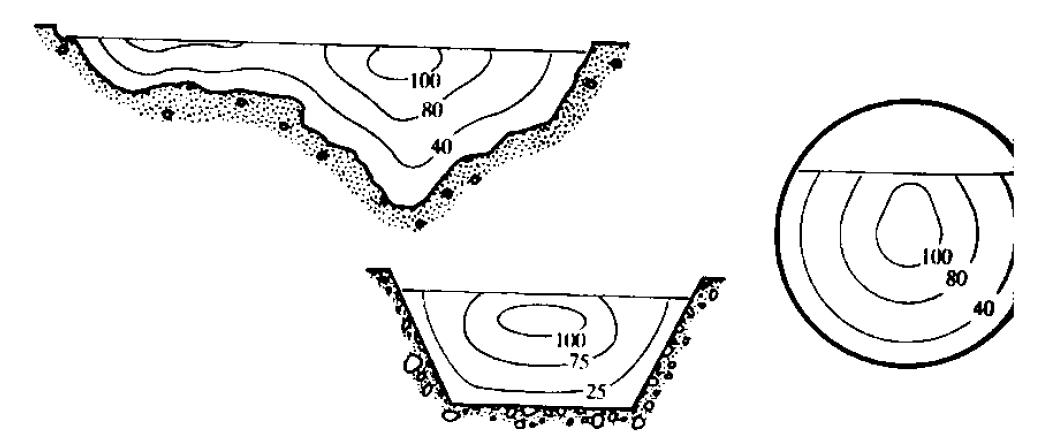
\includegraphics[scale=0.5,angle=2]{./images/fig_142.png}
	\caption{Velocity distributions in open channels, \cite{chadwick}}
	\label{fig:142}
\end{figure}

\subsubsection{Determination of energy and momentum coefficients}

To determine the values of $\alpha$ and $\beta$ the velocity distribution must have been measured (or be know in some way). In irregular channels where the flow may be divided into distinct regions $\alpha$ may exceed 2 and should be included in the Bernoulli equation.

The figure below is a typical example of this situation. The channel may be of this shape when a river is in flood - this is known as a compound channel. 

 \begin{figure}[H]
	\centering
	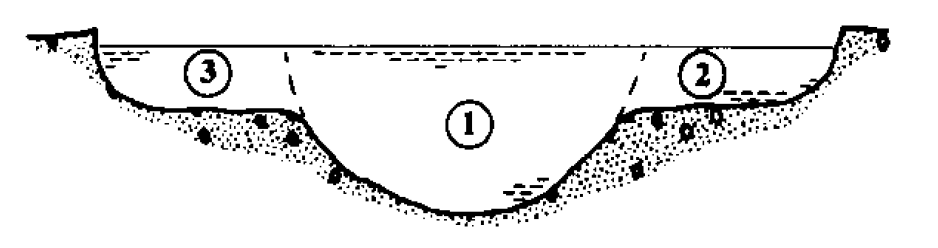
\includegraphics[scale=0.5]{./images/fig_151.png}
	\caption{Compound channel with three region of flow, \cite{chadwick}}
	\label{fig:151}
\end{figure}

If the channel is divided as shown into three regions and making the assumption that $\alpha = 1$ for each then

\begin{equation}
\alpha = \frac{\int u^3 \; dA}{\overline{V}^3 \; A} = \frac{V_1^3 A_1+ V_2^3 A_2+V_3^3 A_3}{\overline{V}^3(A_1+A_2+A_3)} 
\end{equation}
where
\begin{equation}
\overline{V} = \frac{Q}{A} = \frac{V_1 A_1+ V_2 A_2+V_3 A_3}{A_1+A_2+A_3} 
\end{equation} 

\subsection{Laminar and Turbulent flow}

As in pipes , and all flow, the flow in an open channel may be either laminar or turbulent. The criterion for determining the type of flow is the Reynolds Number, $R_e$.

For pipe flow (where $D$ is pipe diameter)
\begin{equation}
R_e = \frac{\rho V D}{\mu} = \frac{VD}{\nu}
\label{eq:re}
\end{equation} 
And the limits for reach type of flow are
\begin{align*}
\text{Laminar}&:  R_{e \text{ pipe}} < 2000 \\
\text{Turbulent}&:  R_{e \text{ channel}} > 4000
\end{align*}

If we take the characteristic length as the hydraulic radius $R = A/P$ then for a pipe \underline{flowing full} 
\begin{equation*}
R = \frac{\pi D^2/4}{\pi D}=\frac{D}{4} 
\end{equation*}
and
\begin{equation}
R_e = \frac{\rho V R}{\mu}=\frac{\rho V}{\mu}\frac{D}{4} = \frac{R_{e  \text{ pipe}}}{4} 
\end{equation}


So for an open channel the limits for each type of flow become
\begin{align*}
\text{Laminar}&:  R_{e \text{ channel}} < 500 \\
\text{Turbulent}&:  R_{e \text{ channel}} > 1000
\end{align*}


In practice the limit for turbulent flow is not so well defined in channel as it is in pipes and so 2000 is often taken as the threshold for turbulent flow.

We can draw further from pipe flow analysis to look at the effect of friction. Taking the Darcy-Wiesbach formula for head loss due to friction in a pipe in turbulent flow 

\begin{equation}
h_f = \frac{4fLV^2}{2gD}
\end{equation}

and make the substitution for hydraulic radius $R = D/4 $,
and if we put the bed slope $S_o = L/h_f$ then

\begin{align}
 S_o = \frac{L}{h_f} \nonumber \\
 S_o = \frac{4fV^2}{2g \; 4R}
\end{align}
 
and
\begin{equation}
\lambda = \frac{8gRS_o}{V^2} \qquad \qquad f = \frac{2gRS_o}{V^2}
\end{equation}

  

The \textit{Colebrook-White}  equation gives the $f - R_e$ relationship for pipes, putting in $R=D/4$ the equivalent equation for open channel is

 \begin{equation}
\frac{1}{\sqrt{f}} = -4 \log_{10} \left(\frac{k_s}{14.8 R}+\frac{1.26}{R_e \sqrt{f}}\right)
 \end{equation}
which can be written for $\lambda - R_e$ relationship (using $\lambda = 4f$)
 \begin{equation}
\frac{1}{\sqrt{\lambda}} = -2 \log_{10} \left(\frac{k_s}{3.7 R}+\frac{2.51}{R_e \sqrt{\lambda}}\right)
\end{equation}

where $k_s$ is the \textit{effective roughness} height

A chart of the $\lambda - R_e$ relationship for open channels can be drawn using this equation but its practical application is not clear. In pipes this relationship is useful but due to the more complex flow pattern and the extra variable (as hydraulic radius, $R$, varies with depth and channel shape) then it is difficult to apply to a particular channel. The general approach is also questionable as there has been no account taken for a free surface which considerably change velocity distributions causing frictional resistance to be much less uniform in open channels than in pipes. 

In practice flow in open channels is usually in the rough turbulent zone and consequently simpler friction formulae may be applied to relate frictional losses to velocity and channel shape.

\subsection{The Froude number}
\label{sec:fr}
The Froude number is defined for channels as:
\begin{equation}
F_r = \frac{V}{\sqrt{gD_m}}
\label{eq:fr}
\end{equation} 
Its physical significance is the ratio of inertial forces to gravitational forces squared
\begin{equation*}
F_r^2 = \frac{\text{initertial force}}{\text{gravitational force}}
\label{eq:fr22}
\end{equation*}
It can also be interpreted as the ratio of water velocity to wave velocity
\begin{equation*}
F_r = \frac{\text{water velocity}}{\text{wave velocity}}
\label{eq:fr2}
\end{equation*}

This is an extremely useful non-dimensional number in open-channel hydraulics.


Although these terms will be defined later,  it is useful to state them here: the value of  $F_r$ determines the \textbf{regime} of flow - sub, super or critical (see later), and the direction in which disturbances travel. These may be summarised as:
\begin{table}[H]
	\centering
	\begin{tabular}{cl}
		$F_r < 1$ &  \textbf{sub-critical} \\
		& water velocity $>$ wave velocity \\
		& upstream levels \textbf{affected} by downstream levels \\
		\noalign{\vskip 2mm} 
		$F_r = 1$ & \textbf{critical} \\
		\noalign{\vskip 2mm} 
		$F_r > 1$ & \textbf{super-critical} \\
		& water velocity $<$ wave velocity \\
		& upstream levels \textbf{NOT affected} by downstream levels \\ 
	\end{tabular}
	%\caption*{Froude number interpretation}
	\label{tab:1111}
\end{table}

\newpage
\section{Uniform Flow in Open Channels}
\subsection{Uniform flow and the Development of Friction formulae}

When uniform flow occurs gravitational forces exactly balance the frictional resistance forces which apply as a shear force along the boundary (channel bed and walls).

\begin{figure}[H]
	\centering
	%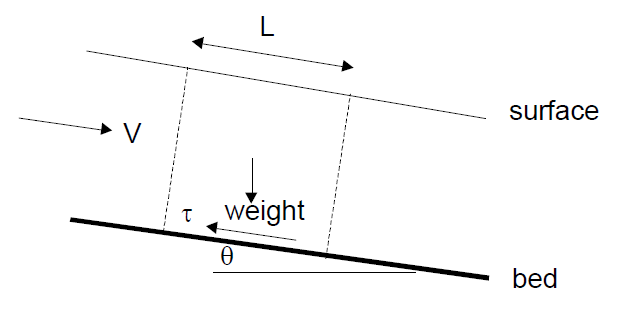
\includegraphics[scale=0.5]{./images/fig_171.png}
	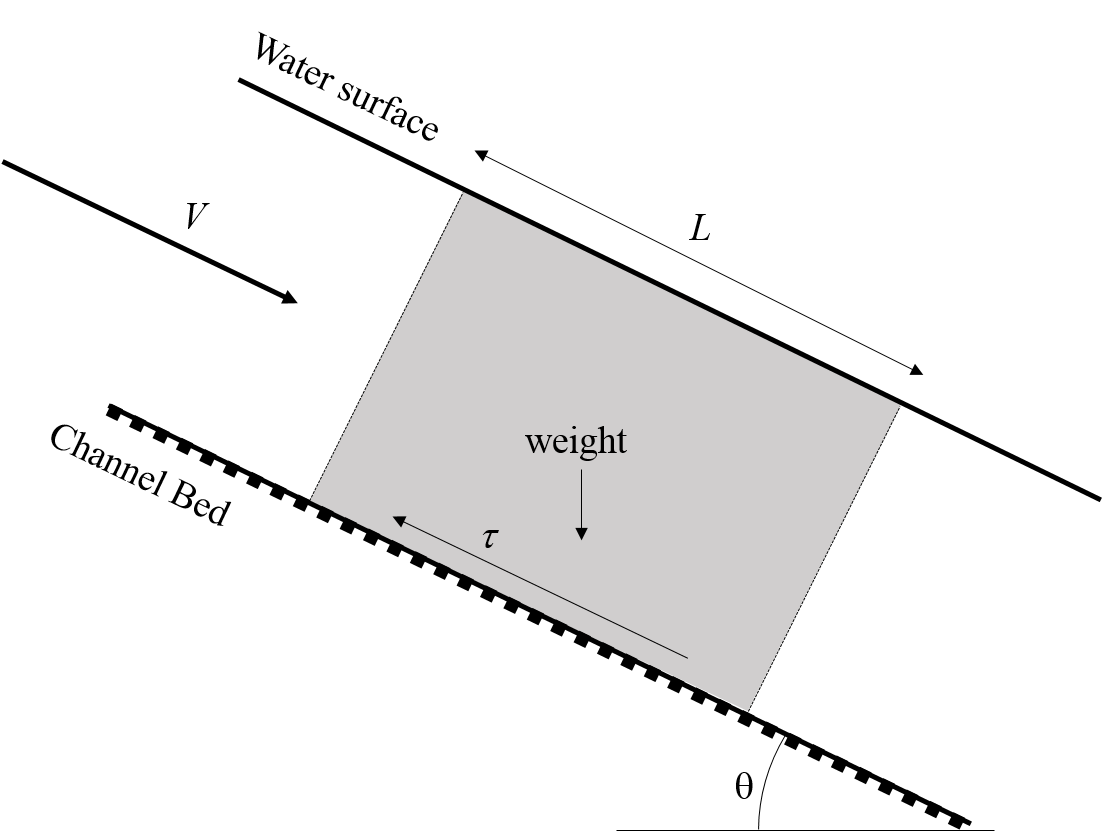
\includegraphics[scale=0.5]{./images/uniform_flow_section_2018.png}
	\caption{Forces on a channel length in uniform flow}
	\label{fig:171}
\end{figure} 
Considering figure \ref{fig:171}, the gravity force resolved in the direction of flow is

\begin{equation}
\text{gravity force} = \rho g A L \sin \theta
\end{equation}
 

and the boundary shear force resolved in the direction of flow is 

\begin{equation}
\text{shear force} = \tau_o P L
\end{equation}
 

In uniform flow these balance
 \begin{equation}
  \tau_o P L = \rho g A L \sin \theta
 \end{equation}
 


Considering a channel of small slope, then
 \begin{equation}
\sin \theta \approx \tan \theta = S_o
\end{equation}


So

 \begin{equation}
\tau_o = \frac{\rho g A S_o}{P} = \rho g R S_o
\label{eq:tau_o}
\end{equation}

\subsubsection{The Chezy equation}

If an estimate of $\tau_o$ can be made then we can make use of Equation \ref{eq:tau_o}.

If we assume the state of rough turbulent flow then we can also make the assumption the shear force is proportional to the flow velocity squared i.e.

 \begin{align*}
\tau_o &\propto V^2 \\
\tau_o &= K V^2
\end{align*}
 

Substituting this into equation \ref{eq:tau_o} gives


\begin{equation}
V = \sqrt{\frac{\rho g}{K}R S_o}
\end{equation} 

Or grouping the constants together as one equal to $C$
\begin{equation}
V = C\sqrt{R S_o}
\label{eq:chezy_v}
\end{equation} 

This is the Chezy equation and the $C$ the 'Chezy $C$'

In terms of $Q = (=AV)$ this is simply
\begin{equation}
Q = AC\sqrt{R S_o}
\label{eq:chezy_q}
\end{equation}

Because the $K$ is not constant the $C$ is not constant but depends on Reynolds number and boundary roughness (see discussion in previous section).

The relationship between $C$ and $\tau$ is easily seen be substituting equation \ref{eq:chezy_v} into the Darcy-Wiesbach equation written for open channels and is
\begin{equation}
C = \sqrt{\frac{2 g}{f}}
\end{equation} 
\subsection{The Manning equation}
A very many studies have been made of the evaluation of C for different natural and manmade channels. These have resulted in today most practising engineers use some form of this relationship to give $C$:

\begin{equation}
C = \frac{R^{1/6}}{n}
\label{eq:chezy_manning}
\end{equation}  

This is known as Manning's formula, and the $n$ as Manning's $n$.

Substituting equation \ref{eq:chezy_v} in to \ref{eq:chezy_manning} gives velocity of uniform flow:
\begin{equation}
V = \frac{R^{2/3}S_o^{1/2}}{n}
\label{eq:manning_v}
\end{equation} 
Or in terms of discharge
\begin{equation}
Q = \frac{1}{n}\frac{A^{5/3}}{P^{2/3}}S_o^{1/2}
\label{eq:manning_q} %eq 1.11
\end{equation} 


\textbf{Note:} \\
Several other names have been associated with the derivation of this formula - or ones similar and consequently in some countries the same equation is named after one of these people. Some of these names are; Strickler, Gauckler, Kutter, Gauguillet and Hagen.

The Manning's $n$ is also numerically identical to the Kutter $n$.

The Manning equation has the great benefits that it is simple, accurate and now due to it long extensive practical use, there exists a wealth of publicly available values of $n$ for a very wide range of channels.

Below is a table of a few typical values of Manning's $n$

\begin{table}[H]
	\centering
	\begin{tabular}{l|c|c}
		\hline
\textbf{Channel type}&\textbf{Surface material and form}&\textbf{Manning's $n$ range }\\
\hline
%\noalign{\vskip 2mm} 
River&earth, straight&0.02-0.025\\
&earth, meandering&0.03-0.05\\
&gravel (75-150mm), straight&0.03-0.04\\
&gravel (75-150mm), winding&0.04-0.08\\
\hline
unlined canal&earth, straight&0.018-0.025\\
&rock, straight&0.025-0.045\\
\hline
lined canal&concrete&0.012-0.017\\
\hline
lab. models&mortar&0.011-0.013\\
&Perspex& 0.009\\
\hline
\end{tabular}
\end{table}
	
\subsubsection{Conveyance}
Channel conveyance, K, is a measure of the carrying capacity of a channel. The $K$ is really an agglomeration of several terms in the Chezy or Manning's equation:
\begin{align}
Q &= AC\sqrt{R S_o} \nonumber \\
&= KS_o^{1/2}
\label{eq:manning_conveyance}
\end{align} 
 So
\begin{equation}
K = ACR^{1/2} = \frac{A^{5/3}}{n P^{2/3}}
\label{eq:conveyance}
\end{equation} 

Use of conveyance may be made when calculating discharge and stage in compound channels and also calculating the energy and momentum coefficients in this situation.

\subsection{\textit{Efficient} Uniform Flow Channels }

The design of a rigid (\emph{i.e.}, non-erodible) surface
open channel should be such that it is capable of carrying
maximum discharge with minimum excavation, construction, and
lining costs. This suggests that the designed
channel should have maximum hydraulic radius for a given
area or minimum perimeter for the given area since hydraulic
radius equals $A/P$. Therefore, a circular or semi-circular
section is the most efficient section. The adoption of
circular channel section is usually not feasible for sections larger than when a pipe could be used, due to the
difficulties of construction to achieves stable earth slopes
and other practical considerations. Hence, the designer has
to determine the most efficient section of a given shape. 
Considering a trapezoidal channel section, Fig. \ref{fig:section_trap_2018}, the
area of flow section $A$ and the wetted perimeter $P$ are given as
\begin{equation}
A = By + sy^2
\label{eq:1281}
\end{equation}
\begin{equation}
P = B +2y \sqrt{1 + s^2}
\label{eq:1282}
\end{equation}
Here,
\begin{equation*}
s = \cot \theta \qquad \qquad \text{or }  \qquad \qquad \frac{1}{s}= \tan\theta
\end{equation*}

\begin{figure}[H]
	\centering
	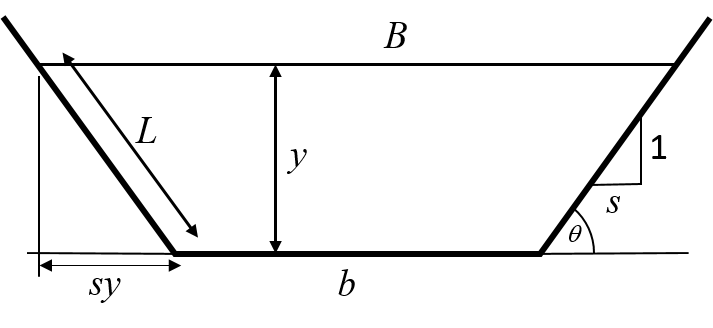
\includegraphics[width=8cm]{./images/section_trap_2018_a.png}
	\caption{A trapezoidal channel section}
	\label{fig:section_trap_2018}
\end{figure}
On substituting the value of $B$ obtained from Eq. \ref{eq:1281}
into Eq. \ref{eq:1282}, one gets
\begin{equation}
P = \frac{A}{y} - sy +2y \sqrt{1 + y^2}
\label{eq:1283}
\end{equation}	
To minimize $P$, evaluate $dP/dy$ with $A$ and $s$ constant
and set $dP/dy$ equal to zero. Therefore, 
\begin{equation*}
\frac{dP}{dy} = -\frac{A}{y^2} - z + 2 \sqrt{1 + s^2} = 0
\end{equation*}
or
\begin{equation}
A = y^2 \left [ 2 \sqrt{1 + s^2} - s \right ]
\label{eq:1284}
\end{equation}
Substituting the value of $A$ in Eq. \ref{eq:1284}, one gets 

\begin{equation*}
By + sy^2 = y^2 \left [ 2 \sqrt{1 + s^2} - s \right ]
\end{equation*}
$\therefore$
\begin{equation}
B = 2y  \left [ \sqrt{1 + s^2} - s \right ]
\label{eq:1285}
\end{equation}
Likewise, substituting the value of $A$ from Eq. \ref{eq:1284}in
Eq. \ref{eq:1283}, one gets

\begin{equation*}
P = y \left [ 2 \sqrt{1 + s^2} - s \right ] - sy + 2y \sqrt{1 + y^2}
\end{equation*}
or
\begin{equation}
P = 4y \sqrt{1 + s^2} - 2sy = 2y\left [ 2 \sqrt{1 + s^2} - s \right ]
\label{eq:1286}
\end{equation}
Thus,
\begin{equation}
R = \frac{A}{P} = \frac{y}{2}
\label{eq:1287}
\end{equation}
Equation  \ref{eq:1287} indicates that for any side slope $\theta$, 
the most efficient uniform flow channel of trapezoidal
shape would be the one for which hydraulic radius is
half the depth of flow. 

For a \textbf{rectangular} section, $\theta =$ 90 or $s=$ 0.
Therefore, the most efficient rectangular channel section
would be the one for which 
\begin{equation*}
A = 2y^2
\label{eq:1288}
\end{equation*}
\begin{equation}
P = 4y
\label{eq:1289}
\end{equation}
\begin{equation}
R = y/2
\label{eq:12810}
\end{equation}
and
\begin{equation}
B = 2y
\label{eq:12811a}
\end{equation}
To obtain the depth of flow for the most efficient section,
these equations must be solved in conjunction with
the Manning's equation.

Equations \ref{eq:1284}, \ref{eq:1287} are valid for any value of $s$.
The best value of $s$ for given $y$ and $A$ can be obtained
by setting $dP/ds$, evaluated from Eq. \ref{eq:1283}, equal to zero. 
\begin{equation*}
\frac{dP}{ds} = -y +2y\left [ \frac{1}{2} \frac{1}{\sqrt{1 + s^2}} \right ] 2s = 0
\end{equation*}
$\therefore$
\begin{equation*}
2s = \sqrt{1 + s^2}
\end{equation*}
$\therefore$
\begin{equation*}
s = \frac{1}{\sqrt{3}} = \cot \theta \qquad \qquad \text{or} \qquad\qquad \frac{1}{s} = \tan \theta = \sqrt{3}
\end{equation*}
$\therefore$
\begin{equation*}
\theta = 60^\circ
\end{equation*}
Thus, the maximum-flow trapezoidal section would be half of a hexagon.

Similarly, one can show that a circular channel section
running partially full would perform best when the depth of
flow is half the diameter. Geometric elements of the most
efficient channel sections of some selected shapes are given
in Table \ref{tab:1281}. Obviously, the semi-circular open channel
section is the best of all possible channel sections as it
gives minimum wetted perimeter for a given area of flow
section. However, the percentage increase in discharge for
semicircular section, compared to that in semi-hexagonal
section, is only small.

\begin{table}[H]
	\centering
	\begin{tabular}{ l llllll }
		\hline
		Cross-section & Normal & Area,  & Wetted  & Hydraulic  & Water surface  & Hydraulic \\
		& depth, $y_n$ & $A$ & perimeter, $P$ & radius, $R$ &  width, $B$ & depth, $D$\\
		\hline 
		Rectangular & $0.917 (Qn/\sqrt{S})^{3/8}$ & $2y^2$ & $4y$ & $0.500 y$ & $2y$ & $y$\\
		Triangle & $1.297 (Qn/\sqrt{S})^{3/8}$ & $y^2$ & $2.83 y$ & $0.354 y$ & $2y$ & $0.500y$\\
		(side slope 1:1) &  &  &  &  &   & \\
		Trapezoid  & $0.968 (Qn/\sqrt{S})^{3/8}$ & $1.73 y^2$ & $3.46 y$ & $0.500 y$ & $2.31 y$ & $0.750 y$\\
		(half of hexagon)  &  &  &  &  &   & \\
		Semicircle & $1.000 (Qn/\sqrt{S})^{3/8}$ &  $0.5\pi y^2$ & $\pi y$ & $0.500y$ & $2y$ & $0.250 \pi y$ \\
		Parabola  & $0.937 (Qn/\sqrt{S})^{3/8}$ & $1.89 y^2$ & $3.77 y$ & $0.500 y$ & $2.83 y$ & $0.667 y$\\
		$B  =  2\sqrt{2y}$ &  &  &  &  &  &   \\
		\hline
	\end{tabular}
	\caption{Geometric elements of the most efficient
		hydraulic sections \cite{french94}}
	\label{tab:1281}
\end{table}

\subsection{Computations in uniform flow}

We can use Manning's formula for discharge to calculate steady uniform flow. Two calculations are usually performed to solve uniform flow problems.
\begin{enumerate}
	\item Discharge from a given depth
	\item Depth for a given discharge
\end{enumerate}
In \underline{steady uniform flow the flow depth is know as normal depth}.

As we have already mentioned, and by definition, uniform flow can only occur in channels of constant cross-section (prismatic channels) so natural channel can be excluded. However we will need to use Manning's equation for gradually varied flow in natural channels - so application to natural/irregular channels will often be required.

\subsubsection{Uniform flow example 1 - Discharge from depth in a trapezoidal channel}

A concrete lined trapezoidal channel with uniform flow has a normal depth is 2m. 
The base width is $5m$ and the side slopes are equal at 1:2 (v:h, or $s=2$ in table \ref{tab:131})
Manning's $n$ can be taken as $0.015$, 
And the bed slope $S_o = 0.001$

What are:
\begin{enumerate}[label=\alph*]
	\item Discharge ($Q$)
	\item Mean velocity ($V$)
	\item Reynolds number ($R_e$)
\end{enumerate}
Calculate the section properties, using the appropriate geometrical formulae (e.g. table \ref{tab:131})

Area, $A =(b+sy)y$  
\begin{equation*}
A= (5 + 2y)y = 18m^2
\end{equation*}
Wetted perimeter, $P =b+2y\sqrt{1+s^2}$
\begin{equation*}
P= 5 + 2y\sqrt{1+2^2} = 13.94m
\end{equation*}
Use equation \ref{eq:manning_q} to get the discharge
\begin{align*}
Q &= \frac{1}{n}\frac{A^{5/3}}{P^{2/3}}S_o^{1/2} \\
&= \frac{1}{0.015}\frac{18^{5/3}}{13.94^{2/3}}0.001^{1/2}\\
& = 45 m^3/s
\end{align*}
Calculate the mean velocity using the continuity equation:
\begin{equation*}
V= \frac{Q}{A}=\frac{45}{18}=2.5 m/s
\end{equation*}
And the Reynolds, $R_e$, number (remember we use the hydraulic radius $R$  as the length scale), and so using $R=A/P$)
\begin{equation*}
R_e = \frac{\rho V R}{\mu} = \frac{\rho V}{\mu}\frac{A}{P} =\frac{1000 \times 2.5}{1.14\times 10^{-3} }\frac{18}{13.9} = 2.84 \times 10^6
\end{equation*}
This is very large - i.e. well into the turbulent zone - the application of the Manning's equation was therefore valid. 

What solution would we have obtained if we had used the Colebrook-White equation?

Probably very similar as we are well into the rough-turbulent zone where both equations are truly applicable.

To experiment an equivalent $k_s$ value can be calculated for the discharge calculated from $n = 0.015$  and $y = 2m$ [$k_s = 2.225mm$] (Use the Colebrook-White equation and the Darcy-Wiesbach equation of open channels - both given earlier). Then a range of depths can be chosen and the discharges calculated for these $n$ and $k_s$ values. Comparing these discharge calculations will give some idea of the relative differences - they will be very similar.


\subsubsection{Uniform flow example 2 - Depth from Discharge in a trapezoidal channel}

Using the same channel as above, if the discharge is know to be $30m^3/s$ in uniform flow, what is the normal depth?

Again use equation \ref{eq:manning_q} 

Area, $A =(b+sy)y$  \\
Wetted perimeter, $P =b+2y\sqrt{1+s^2}$
\begin{align*}
Q &= \frac{1}{0.015}\frac{((5+2y)y)^{5/3}}{\left(2+2y\sqrt{1+2^2}\right)^{2/3}}0.001^{1/2}\\
30 &= 2.108\frac{((5+2y)y)^{5/3}}{\left(2+2y\sqrt{1+2^2}\right)^{2/3}}
\end{align*}
We need to calculate $y$ from this equation (and remember that this is \textbf{normal depth} so $y = y_n$. 

Even for this quite simple geometry the equation we need to solve for normal depth is complex. 

One simple strategy to solve this is to try some trial values of $y$ and calculate the right hand side of this equation and compare it to $Q (=30)$ on the left. When it equals $Q$ we have the correct $y$. Even though there will be several solutions to this equation, this strategy generally works because we have a good idea of what the depth should be (e.g. it will always be positive and often in the range of $0.5 \text{ to } 10 m$). 

In this case from the previous example we know that at $Q = 45 m^3/s$, $y = 2m$. So at $Q = 30 m^3/s3 then 3y < 2.0m$.

\begin{table}[H]
	\centering
	\begin{tabular}{cc}
		\hline
		Trials of $y$ ($m$) &Discharge $Q$ ($m^3/s$) \\
		\hline
		1.7	&32.7\\
		1.6	&29.1\\
		1.63&	30.1\\
		\hline
	\end{tabular}
	\caption{Trials of $y$}
	\label{tab:ex21}
\end{table}

\subsubsection{Uniform flow example 3 - A compound channel}

If the channel in the above example were to be designed for flooding it may have a section like this:

\begin{figure}[H]
	\centering
	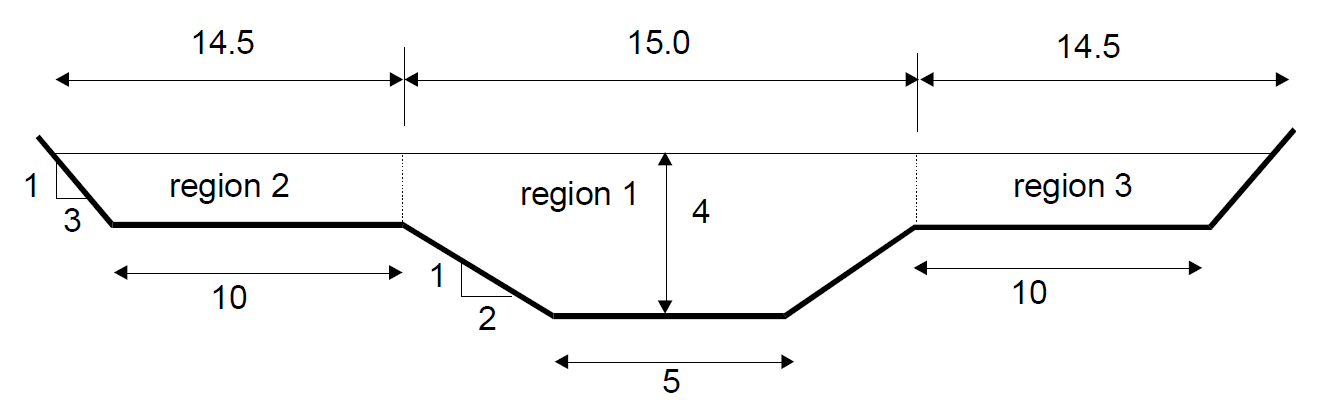
\includegraphics[scale=0.5]{./images/fig_eg41.png}
	\caption{A Compound section}
	\label{fig:eg41}
\end{figure}
When the flow goes over the top of the trapezoidal channel it moves to the "flood plains" so the section allows for a lot more discharge to be carried.

If the flood channels are 10m wide and have side slopes of $1:3$, and the Manning $n$ on these banks is $0.035$, what are
\begin{enumerate}[label=\alph*,noitemsep]
	\item the discharge for a flood level of $4m$?
	\item the energy coefficient ?
\end{enumerate}
First split the section as shown in to three regions (this is arbitrary - left to the engineers judgement). 
Then apply Manning's formula for each section to give three discharge value and the total discharge will be $Q = Q_1 + Q_2 + Q_3$.

Calculate the properties of each region:
\begin{equation*}
A_1 = \left( \frac{5+15}{2}\right)2.5+(15 \times 1.5) = 47.5m^2
\end{equation*}
\begin{equation*}
A_2 = A_3 = \left( \frac{10+14.5}{2}\right)1.5 = 18.38m^2
\end{equation*}
\begin{equation*}
P_1 = 5 + \left(2 \sqrt{5}\times 2.5\right) = 16.18m
\end{equation*}
\begin{equation*}
P_2 = P_3=10 + \left(1.5 \sqrt{10}\times \right) = 14.75m
\end{equation*}
The conveyance for each region may be calculated from equation \ref{eq:conveyance}
\begin{equation*}
K_1 =\frac{47.5^{5/3}}{0.015 \times 16.18^{2/3}} = 6492.5
\end{equation*}
\begin{equation*}
K_2 = K_3 =\frac{18.38^{5/3}}{0.035 \times 14.74^{2/3}} = 608.4
\end{equation*}


And from Equation \ref{eq:manning_q} or Equation \ref{eq:manning_conveyance}
the discharges
\begin{equation*}
Q_1 = \frac{1}{0.015}\frac{47.5^{5/3}}{16.18^{2/3}}0.001^{1/2}
\end{equation*}
or
\begin{equation*}
Q_1 = K_1 0.001^{1/2}= 205.3 m^3/s
\end{equation*}
And
\begin{equation*}
Q_2 = Q_3 = \frac{1}{0.035}\frac{18.38^{5/3}}{14.74^{2/3}}0.001^{1/2}
\end{equation*}
or
\begin{equation*}
Q_2=Q_3 = K_2 0.001^{1/2}= 19.2 m^3/s
\end{equation*}
So
\begin{equation*}
Q = Q_1 + Q_2 + Q_3 = 243.7 m^3/s
\end{equation*}
The velocities can be obtained from the continuity equation:
\begin{equation*}
V_1 = \frac{Q_1}{A_1} = 4.32 m/s
\end{equation*}
\begin{equation*}
V_2 = V_3 = \frac{Q_2}{A_2} = 1.04 m/s
\end{equation*}
And the energy coefficient may be obtained from Equation \ref{eq:alpha}
\begin{equation*}
\alpha = \frac{\int u^3 \; dA}{\overline{V}^3 \; A} = \frac{V_1^3 A_1+ V_2^3 A_2+V_3^3 A_3}{\overline{V}^3(A_1+A_2+A_3)} 
\end{equation*}
where
\begin{equation*}
\overline{V} = \frac{Q}{A} = \frac{V_1 A_1+ V_2 A_2+V_3 A_3}{A_1+A_2+A_3} 
\end{equation*} 
Giving 
\begin{equation*}
\alpha = 1.9
\end{equation*}


This is a \textbf{very high} value of $\alpha$ and a clear case of where a velocity coefficient should be used.

Note that this method does not give completely accurate relationship between stage and discharge because some of the assumption are not accurate. E.g. the arbitrarily splitting in to regions of fixed Manning $n$ is probably not what is occurring in the actual channel. However it will give a good estimate as long as care is taken in choosing these regions.



\newpage
\section{Rapidly Varied Flow}
\subsection{The Application of the Energy equation for Rapidly Varied Flow}

Rapid changes in stage and velocity occur whenever there is a sudden change in cross-section or some obstruction in the channel. This type of flow is termed \textbf{rapidly varied flow}. Typical example are flow over sharp-crested weirs and flow through regions of greatly changing cross-section (Venturi flumes and broad-crested weirs).

Rapid change can also occur when there is a change from super-critical to sub-critical flow (see later) in a channel reach at a hydraulic jump.

In these regions the surface is highly curved and the assumptions of hydro static pressure distribution and parallel streamline do not apply. However it is possibly to get good approximate solutions to these situations yet still use the energy and momentum concepts outlined earlier. The solutions will usually be sufficiently accurate for engineering purposes.

\subsubsection{The energy (Bernoulli) equation}
The figure below shows a length of channel inclined at a slope of $\theta$ and flowing with uniform flow.
 \begin{figure}[H]
 	\centering
 	%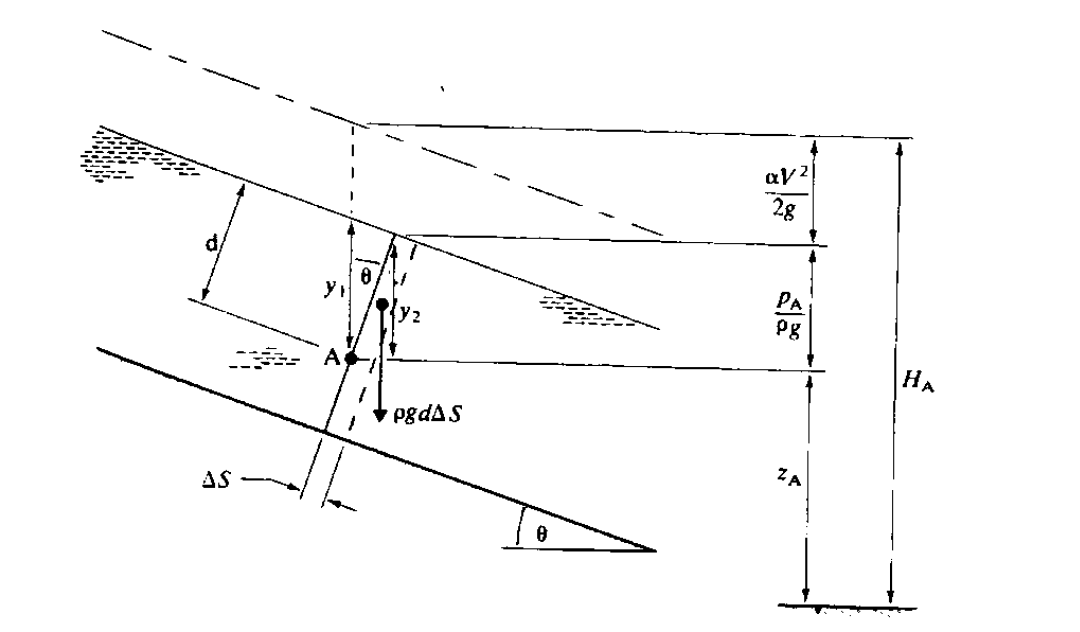
\includegraphics[scale=0.5]{./images/fig_191.png}
 	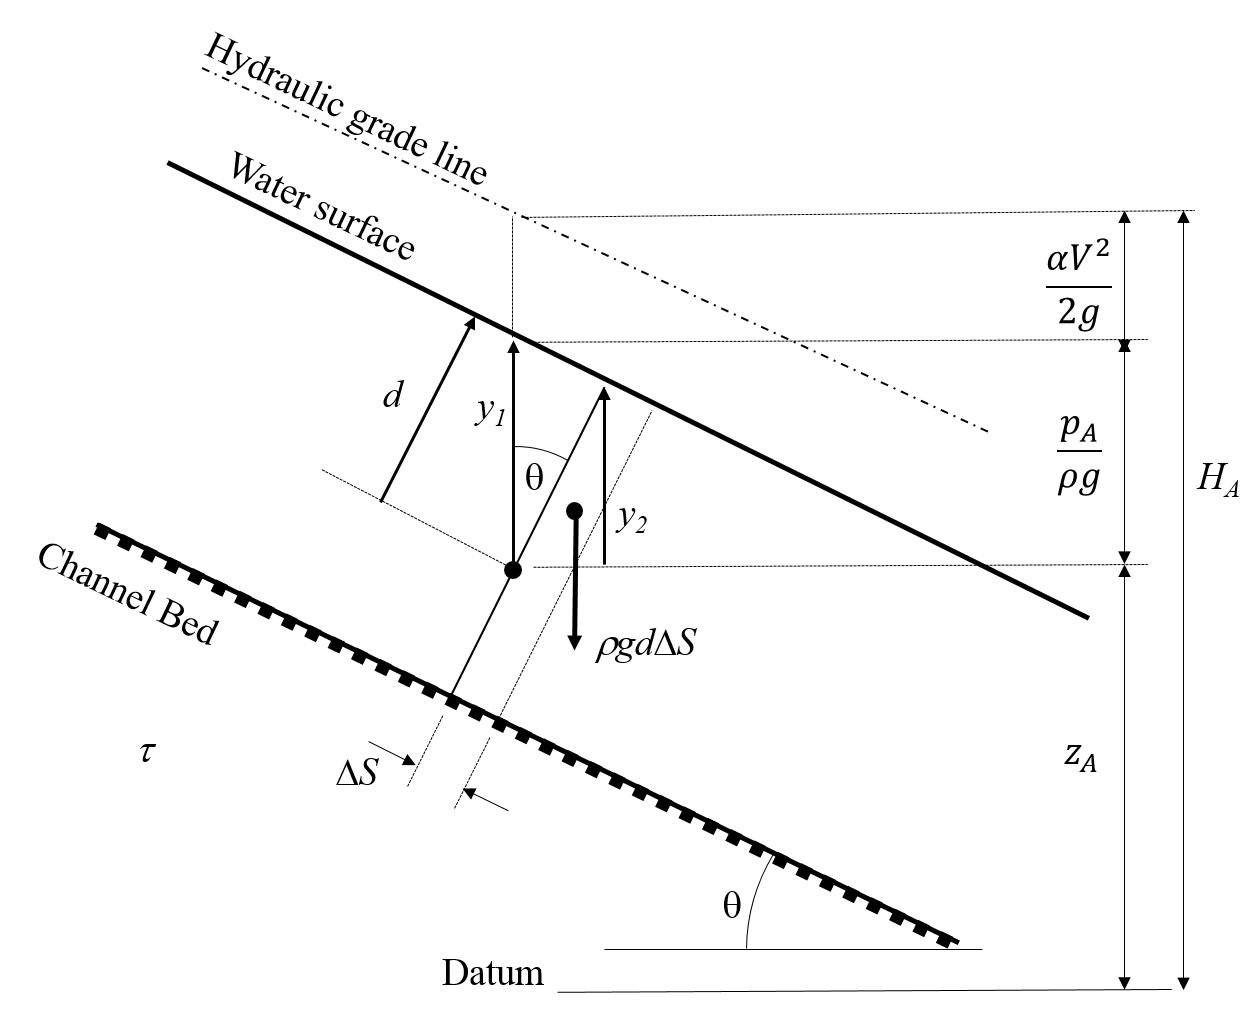
\includegraphics[scale=0.45]{./images/uniform_flow_detail_2018.png}
 	\caption{A channel in uniform flow}
 	\label{fig:191}
 \end{figure} 
Recalling the Bernoulli equation \ref{eq:bernoulli_V}
  \begin{equation*}
 \frac{p}{\rho g}  + \frac{ \alpha V^2}{2g} + z  = \text{constant}
 \label{eq:bernoulli_V2}
 \end{equation*}
And assuming a hydrostatic pressure distribution we can write the pressure at a point on a streamline, $A$ say, in terms of the depth $d$ (the depth measured from the water surface in a direction \textbf{at right angles} to the bed) and the channel slope.
 \begin{equation}
 p_A = \rho g d
 \end{equation}
 In terms of the \textbf{vertical}  distance
  \begin{equation}
d = \frac{y_2}{\cos \theta} = y_1 \cos \theta
\end{equation}
  \begin{equation}
y_2 = y_1 \cos^2 \theta
\end{equation}
So
  \begin{equation}
p_A = \rho g  y_1 \cos^2 \theta
\end{equation} 
So the pressure term in the above Bernoulli equation becomes
  \begin{equation}
\frac{p_A}{\rho g}  = y_1 \cos^2 \theta
\end{equation}

As channel slopes in open channels are generally very small $(1:100 \equiv \theta = 0.57$  and 
$\cos^2 = 0.9999)$ so unless the channel is unusually steep 
   \begin{equation}
 \frac{p_A}{\rho g}  = y_1 
 \end{equation}
And the Bernoulli equation becomes
  \begin{equation}
y  + \frac{ \alpha V^2}{2g} + z  = H
\label{eq:bernoulli_channel} %1.14
\end{equation}


\subsubsection{Flow over a raised hump - Application of the Bernoulli equation}

We will look at the example of steady uniform flow that is interrupted by a raised bed level as shown. If the upstream depth, $y_1$ and discharge, $Q$ are known we can use equation \ref{eq:bernoulli_channel} and the continuity equation to give the velocity and depth of flow over the raised hump of height $\Delta z$.

  \begin{figure}[H]
 	\centering
 	%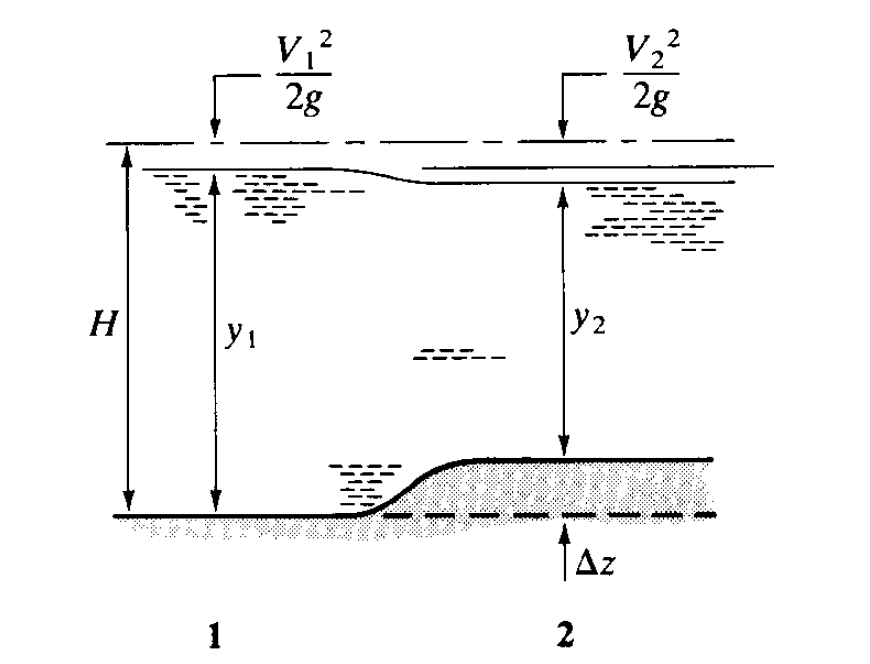
\includegraphics[scale=0.5]{./images/fig_192.png}
 	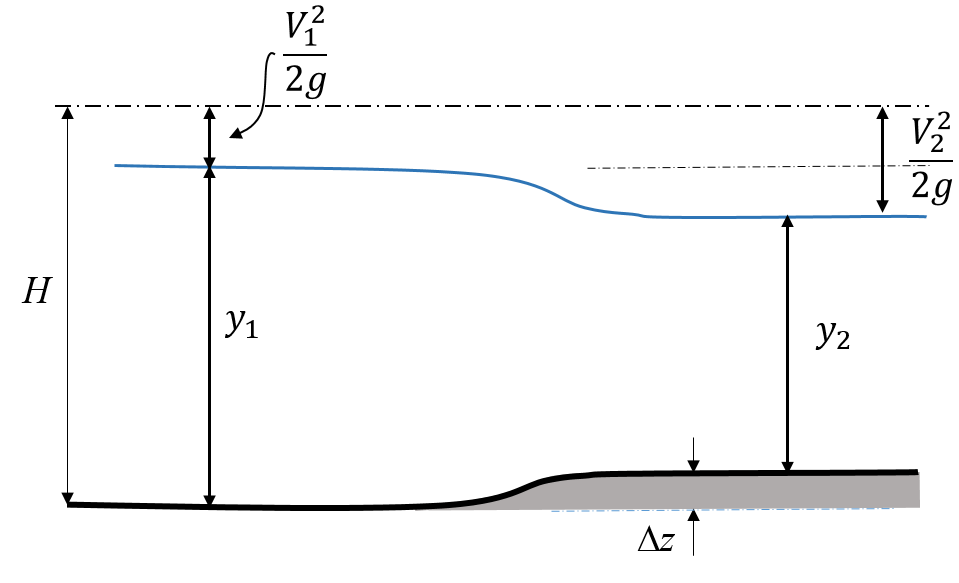
\includegraphics[scale=0.6]{./images/hump_1_2018.png}
 	\caption{Uniform flow interrupted by a raised hump, \cite{chadwick}}
 	\label{fig:192}
 \end{figure} 

Apply the Bernoulli equation between sections 1 and 2. (And assume a horizontal, rectangular channel $z_1 = z_2$  of width $B$. And take $\alpha = 1$)
  \begin{equation}
y_1  + \frac{  V_1^2}{2g}   = y_2  + \frac{  V_2^2}{2g}  + \Delta z
\label{eq:bernoulli_hump1}
\end{equation}

Using the continuity equation 
   \begin{equation}
 V_1 A_1 = V_2 A_2 = Q 
 \label{eq:continuity}
 \end{equation}
For a rectangular prismatic channel $A=By$, so
   \begin{equation}
V_1 y_1 = V_2 y_2 = \frac{Q}{B} = q 
\label{eq:continuity_q}
\end{equation}
Where $q$ is referred to as the \textit{flow per unit width}. 

Substitute Eqn \ref{eq:continuity_q} into the Bernoulli equation, Eq \ref{eq:bernoulli_hump1} to give:
   \begin{equation}
 y_1  + \frac{ q^2}{2gy_1^2}   = y_2  + \frac{ q^2}{2gy_2^2}  +\Delta z
 \label{eq:bernoulli_hump2}
 \end{equation}
rearranging:
   \begin{equation}
2gy_2^3  + y_2^2 \left(2g\Delta z - 2g y_1 - \frac{q^2}{y_1^2}\right) + q^2=0
\label{eq:bernoulli_hump3}
\end{equation}
 

Thus we have a cubic with the only unknown being the downstream depth, $y_2$. There are three solutions to this - only one is correct for this situation. We must find out more about the flow before we can decide which it is.

\subsubsection{Specific Energy}

The extra information needed to solve the above problem can be provided by the specific energy equation. 

Specific energy, $E_s$,  is defined as the energy of the flow with reference to the channel bed as the datum:

   \begin{equation}
E_s = y  + \frac{ \alpha V^2}{2g}
\label{eq:specific_energy}
\end{equation} 

For steady flow this can be written in terms of discharge $Q$
   \begin{equation}
E_s = y  + \frac{ \alpha (Q/A)^2}{2g}
\label{eq:specific_energyQ}
\end{equation} 

 


For a rectangular channel of width $b$, $Q/A = q/y$
   \begin{align*}
E_s &= y  + \frac{ \alpha q^2}{2gy^2}\\
(E_s - y)y^2 &= \frac{\alpha q^2}{2g} = \text{constant} \\
(E_s - y) &= \frac{\text{constant}}{y^2}
\label{eq:specific_energy_rect_q}
\end{align*} 
 
This is a cubic in $y$. It has three solutions but only two will be positive, both of these are \textit{possible}. Discard the negative solution (as it is unphysical).
 
\subsubsection{Flow over a raised hump - revisited. \\Application of the Specific energy equation.}

The specific energy equation may be used to solve the raised hump problem. The figure below shows the hump and stage drawn alongside a graph of Specific energy $E_s$ against $y$.

   \begin{figure}[H]
 	\centering
 	%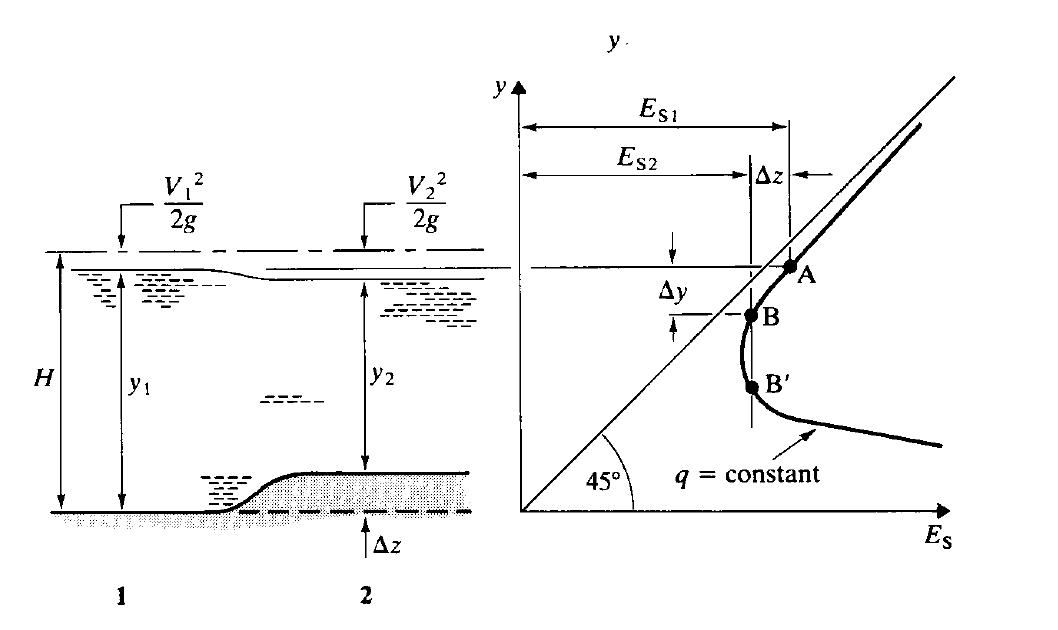
\includegraphics[scale=0.5]{./images/fig_194.png}
 	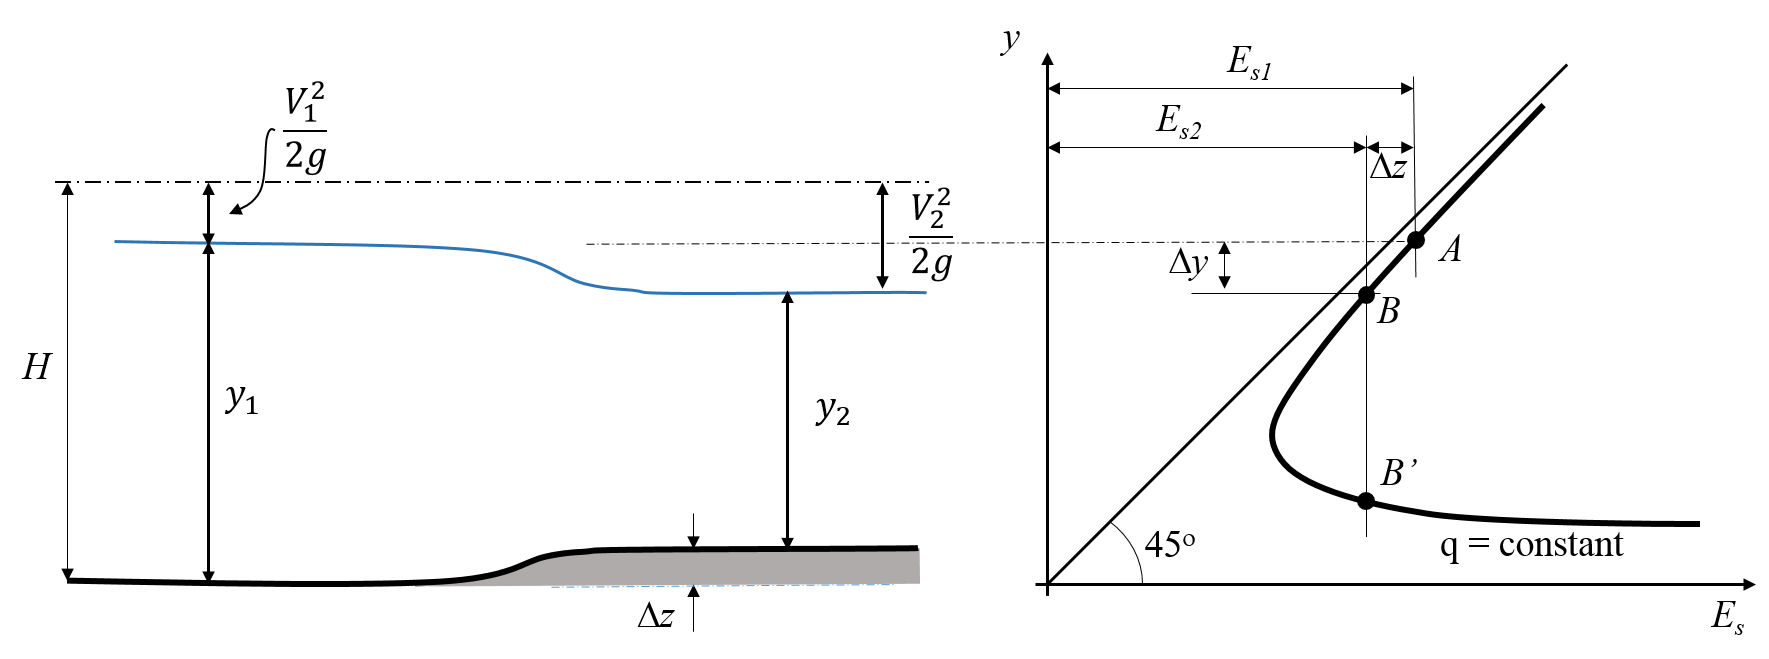
\includegraphics[scale=0.6]{./images/hump_2_Es_2018.png}
 	\caption{Raised bed hump and corresponding graph of specific energy, \cite{chadwick}}
 	\label{fig:194}
 \end{figure} 


The Bernoulli equation was applied earlier to this problem and equation (from that example) \ref{eq:bernoulli_hump1} may be written in terms of specify energy:

  \begin{align}
y_1  + \frac{  V_1^2}{2g}   &= y_2  + \frac{  V_2^2}{2g}  + \Delta z \nonumber \\
E_{s1} &= E_{s2} + \Delta z
\end{align}
 

These points are marked on the figure. Point A on the curve corresponds to the specific energy at point 1 in the channel, but Point B \textbf{or} Point B' on the graph may correspond to the specific energy at point 2 in the channel.

All point in the channel between point 1 and 2 \textbf{must}  lie on the specific energy curve between point A and B or B'. To reach point B' then this implies that $E_{S1} - E_{S2} > \Delta z$ which is not physically possible. So point B on the curve corresponds to the specific energy and the flow depth at section 2.

\subsection{Example of the raised bed hump.}

A rectangular channel with a flat bed and width $5m$ and maximum depth $2m$ has a discharge of $10m^3/s$. The normal depth is $1.25 m$. What is the depth of flow in a section in which the bed rises $0.2m$  over a distance $1m$.

Assume frictional losses are negligible so we can use this expression
\begin{equation*}
E_{s1}= E_{s2}+\Delta z
\end{equation*}
Entering the values given in the question
\begin{align*}
E_{s1} &= 1.25 + \frac{\left(\frac{10}{1.25 \times 5}\right)^2}{2g}=1.38 \\
E_{s2} &= y_2 + \frac{\left(\frac{10}{5 \times y_2}\right)^2}{2g}=y_2 + \frac{0.2039}{y_2^2} \\
\end{align*}
using
\begin{equation*}
E_{s1} = E_{s2} + \Delta z 
\end{equation*}
\begin{align*}
1.38 &= y_2 + \frac{0.2039}{y_2^2} +0.2 \\
1.18 &= y_2 + \frac{0.2039}{y_2^2} = E_{s2} \\
\end{align*}
This can be solved by a trial and error method with values = $y_2$ until the ex[pression is  close to $1.18 (=E_{s2})$:

\begin{table}[H]
	\centering
	\begin{tabular}{cc}
		\hline
		Trials of $y_2$ $(m)$ & $E_{s2}$ $(m$) \\
		\hline
		0.9 & 1.15 \\
		1.0 & 1.2 \\
		0.96 & 1.18 \\
		\hline
	\end{tabular}
	\caption{Trials of $y_2$}
	\label{tab:ex31}
\end{table}
i.e. the depth of the raised section is $0.96m $, or the water level (stage) is $1.16m \; (=0.96+0.2)$ a drop of $9cm$ when the bed has been raised $20cm$.

\subsection{Critical, Sub-critical and Super-critical flow}
\label{sec:Es}
The specific energy change with depth was plotted above for a constant discharge $Q$, it is also possible to plot a graph with the specific energy fixed and see how $Q$ changes with depth. These two forms are plotted side by side below.
 
    \begin{figure}[H]
 	\centering
 	%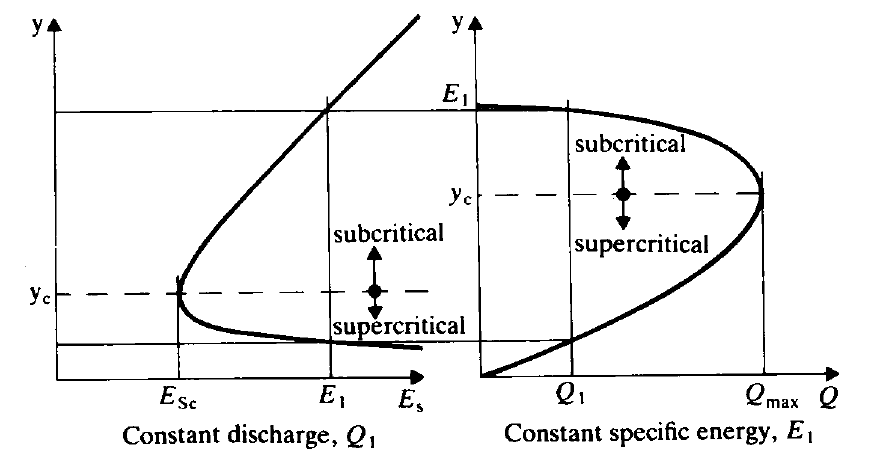
\includegraphics[scale=0.5]{./images/fig_1101.png}
 	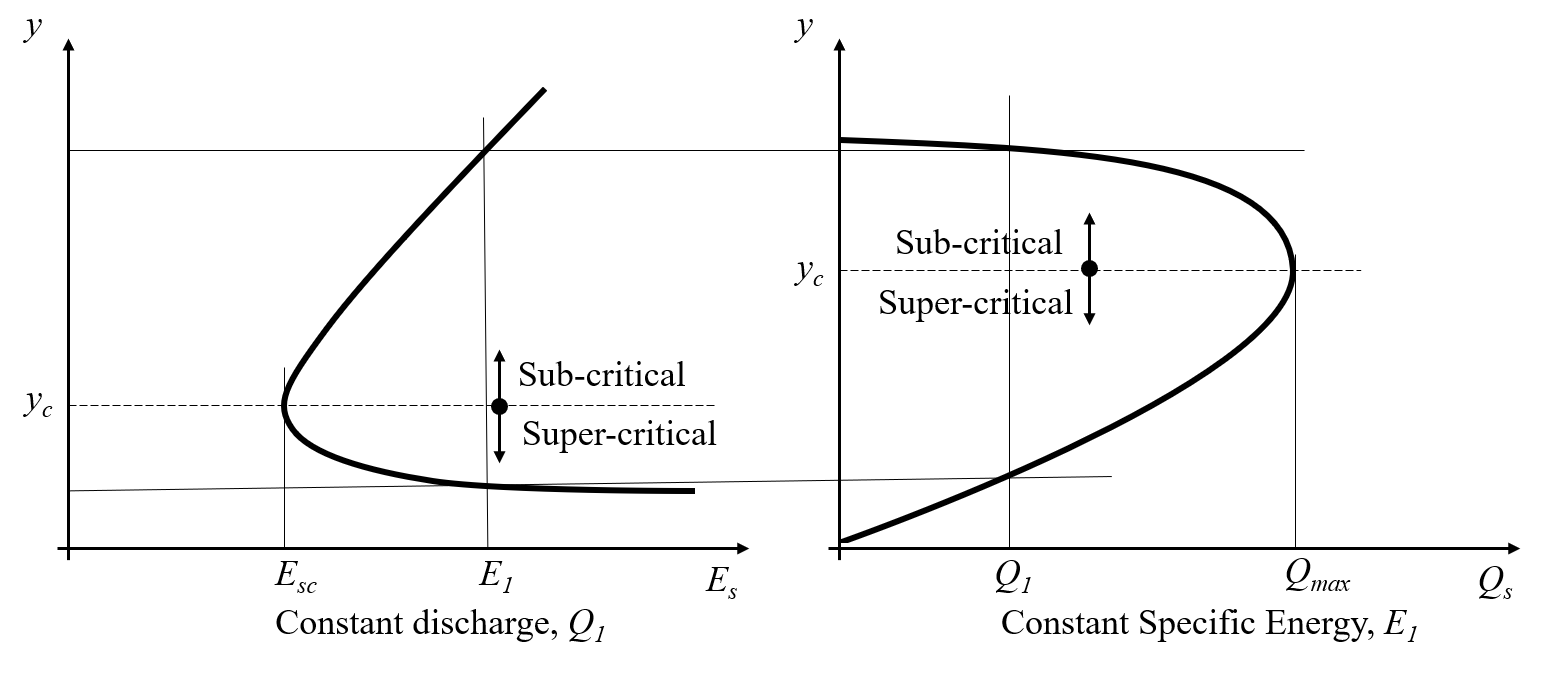
\includegraphics[scale=0.5]{./images/Es_Q_2018.png}
 	\caption{Variation of Specific Energy and Discharge with depth, \cite{chadwick}}
 	\label{fig:1101}
 \end{figure} 
From these graphs we can identify several important features of rapidly varied flow.

\textbf{For a fixed discharge:}\\
\begin{enumerate}
	\item The specific energy is a minimum, $E_{sc}$, at depth $y_c$, \\
This depth is known as \textbf{ critical depth}.
\item For all other values of $E_s$ there are two possible depths. \\
These are called \textbf{alternate depths} (or \textbf{conjugate depths}):
\begin{align*}
\textbf{subcritical flow:  } y > y_c \\
\textbf{supercritical flow:  } y < y_c
\end{align*}
\end{enumerate}


\textbf{For a fixed Specific energy}\\
\begin{enumerate}
	\item The discharge is a maximum at critical depth, $y_c$.
	\item For all other discharges there are two possible depths of flow for a particular $E_s$\\
i.e. There is a sub-critical depth and a super-critical depth with the same $E_s$.
\end{enumerate}

An equation for critical depth can be obtained by setting the differential of $E_s$ to zero:
\begin{equation}
E_s = y \frac{\alpha (Q/A)^2}{2g}
\end{equation}
Setting $dE_s/dy = 0$ gives the turning point
\begin{equation}
\frac{dE_s}{dy} = 0 = 1 + \frac{\alpha Q^2}{2g} \frac{d}{dA}\left(\frac{1}{A^2}\right)\frac{dA}{dy}
\end{equation}
 

Since  $\delta A = B \delta y$, in the limit $dA/dy = B$ and
\begin{align}
0 &= 1 - \frac{\alpha Q^2}{2g}B_c 2 A_c^{-3}  \nonumber \\
\frac{\alpha Q^2 B_c}{gA_c^{3}} &= 1
\label{eq:crit_Q_general} % eq 1.17
\end{align}


For a rectangular channel $Q = qb$, $B = b$ and $A = by$, and taking $\alpha = 1$ this equation becomes
\begin{equation}
y_c = \left(\frac{q^2}{g}\right)^{1/3}
\label{eq:yc_rect}
\end{equation}
as $V_c y_c= q$
\begin{equation}
V_c = \sqrt{gy_c}
\label{eq:crit_vel} %eq 1.18
\end{equation}
Substituting this in to the specific energy equation
\begin{align}
E_{sc} &= y_c + \frac{V_c^2}{2g} \nonumber \\
       &= y_c + \frac{y_c}{2} \nonumber \\
y_c &= \frac{2}{3}E_{sc}
\label{eq:ycrit_esc} %1.19
\end{align}
 
\subsection{Sub and Super Critical Flow Determination and Significance}
\label{sec:fr2}

As first introduced in section \ref{sec:fr}, the Froude number is defined for channels as eqn \ref{eq:fr} and is used primarily to determine whether a flow is sub or super critical:
\begin{equation*}
F_r = \frac{V}{\sqrt{gD_m}}
\label{eq:fr_v2}
\end{equation*} 

The consideration of specific energy has given us another means of determining whether the flow is sub or super-critical by enabling the calculation of the critical depth: eqn \ref{eq:crit_Q_general} in general, or eqn \ref{eq:yc_rect}.

It is worth considering again the significance of sub and super-critical flow.

In super-critical flow the flow velocity is greater than the wave velocity, so the wave cannot travel up-stream. Conversely the wave \textit{can} travel upstream in sub-critical flow. i.e. conditions can change up-stream in sub-critical flow, but they cannot in super-critical flow.

So the value of $F_r$ determines the regime of flow - sub, super or critical, and the direction in which disturbances travel. The summary table from \ref{sec:fr} is repeated again.
\begin{table}[H]
	\centering
	\begin{tabular}{cl}
$F_r < 1$ &  \textbf{sub-critical} \\
& water velocity $>$ wave velocity \\
& upstream levels \textbf{affected} by downstream levels \\
\noalign{\vskip 2mm} 
$F_r = 1$ & \textbf{critical} \\
\noalign{\vskip 2mm} 
$F_r > 1$ & \textbf{super-critical} \\
& water velocity $<$ wave velocity \\
& upstream levels \textbf{NOT affected} by downstream levels \\ 
	\end{tabular}
	\caption*{}
	\label{tab:1111_v2}
\end{table}
Figure \ref{fig:1111} illustrates this for a flow which is sub-critical (top figure) going over a weir, the raised height of the water moves to affect water up-stream. For the (lower figure) super-critical flow down a steep slope forces the flow in the flatter channel down-stream.
\begin{figure}[H]
	\centering
	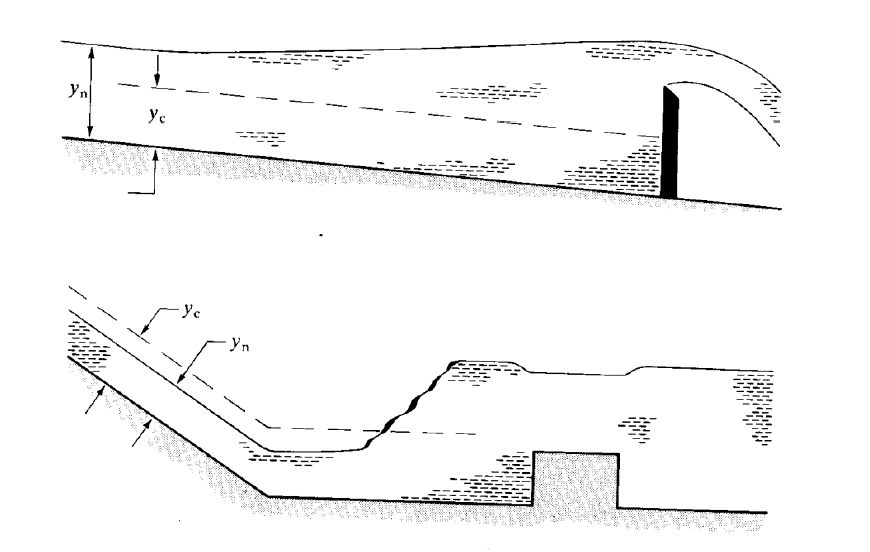
\includegraphics[scale=0.6,angle=2]{./images/fig_1111.png}
	\caption{Sub and super critical flow and transmission of disturbances, \cite{chadwick}}
	\label{fig:1111}
\end{figure} 

\subsection{Specific Force}
While applying momentum principle, Eq. \ref{eq:momentum_gen}, for a
short horizontal reach of a prismatic channel, one can
ignore the external force of friction and the weight
component of water for the reach under consideration. If the
momentum correction factor $\beta $ is also assumed to be
unity, (which is valid for a short, prismatic channel), then Eq. \ref{eq:momentum_gen}  gives 
\begin{equation}
\rho Q (V_2 - V_1) = P_1 - P_2
\label{eq:1341}
\end{equation}
or
\begin{equation*}
M_2 - M_1 = P_1 - P_2
\label{eq:1341a}
\end{equation*}
where $M_1 = \rho Q V_1$ and $M_2 = \rho Q V_2$, and
the hydrostatic forces $P_1$ and $P_2$ may be expressed as, 
\begin{equation}
P_1 = \rho g \bar{z_1} A_1
\label{eq:1342}
\end{equation}
and
\begin{equation}
P_2 = \rho g \bar{z_2} A_2
\label{eq:1343}
\end{equation}
Here, $\bar{z}$ represents the distance of the centroid of the flow
section $A$ below the free surface. Equation \ref{eq:1341}, therefore, yields
or
\begin{equation*}
\rho Q \left ( \frac{Q}{A_2} - \frac{Q}{A_1} \right ) = \rho g \bar{z_1} A_1 - \rho g \bar{z_2} A_2
\end{equation*}
or
\begin{equation}
\frac{Q^2}{g A_1} + \bar{z_1} A_1 = \frac{Q^2}{g A_2} + \bar{z_2} A_2
\label{eq:1344}
\end{equation}
Both sides of Eq. \ref{eq:1344} are similar and, hence, may
be expressed as, say, 
\begin{equation}
F = \frac{Q^2}{g A} + \bar{z} A
\label{eq:1345}
\end{equation}
Here, the term $Q^2 / g A$ is the momentum of the flow (i.e. $\rho Q U$ or $\rho Q^2 / A$) passing through a
flow section of a channel per unit time per unit weight of
the flowing fluid. The second term on the right side of Eq.
\ref{eq:1345}, $\bar{z}A$ represents the hydrostatic force per unit weight
of water. Thus, $F$ is essentially the sum of the two forces per
unit weight of water and, therefore, called the \emph{specific
	force}. Equation \ref{eq:1344} can, accordingly, be written as
\begin{equation*}
F_1 = F_2
%\label{eq:1346}
\end{equation*}
meaning that the specific forces at the end sections of a
channel reach are equal provided that the channel is
horizontal (or the bed slope of the channel is very small)
and the external forces (e.g. friction) acting on the flowing fluid between
the end sections can be ignored. 

\subsection{Application of the Momentum equation for Rapidly Varied Flow}
\subsubsection{Force on Structure in Open Channel Flow}
\label{sec:force_on_struct}
If we consider an obstruction (which could represent any structure, bridge, gate etc.) in a flow, such as that shown in figure \ref{fig:1112a}, we analyse the forces on that obstruction by considering a \textit{control volume} - such as that shown as a dashed box, and condider the momentum change entering and leaving the control volume. (For a short length of channel over a structure, it is common andappropriate to neglect the forces due to the fluid weight and frictional resistance). The rate of change of the momentum gives the \textit{Total} force or \textit{Momentum} force, $M$.
\begin{align*}
M &= \rho Q V_2 - \rho Q V_1 \\
 &= M_2 - M_1\\
 &=\rho Q (V_2 - V_1)
\end{align*}
\begin{figure}[H]
	\centering
	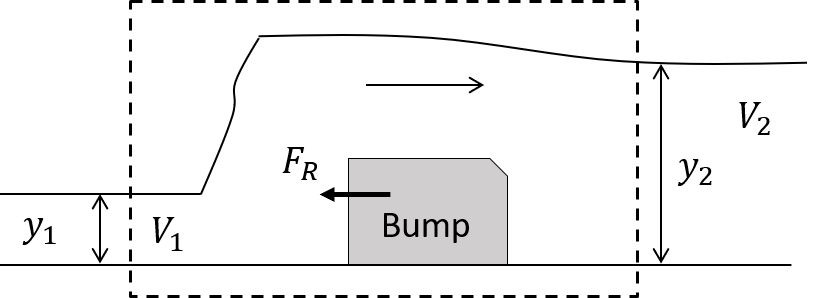
\includegraphics[scale=0.7]{./images/force_on_bump.png}
	\caption{Forces on a structure (obstruction) within Open Channel Flow}
	\label{fig:1112a}
\end{figure} 
The \textit{Pressure} force $P$ is
\begin{align*}
P &= \rho g \bar{z_1} A_1 - \rho g \bar{z_2} A_2 \\
  &= P_1 - P_2 \\
  &= \rho g (\bar{z_1} A_1 - \bar{z_2} A_2)
\label{eq:1112b}
\end{align*}
For a rectangular channel, where $\bar{z} = \frac{y}{2}$ and $A=by$, then
\begin{equation*}
P = \rho g b\frac{1}{2}(y^2_1 - y^2_2)
\label{eq:1112c}
\end{equation*}
We can equatethe total force to the pressure plus reaction force
\begin{align*}
M &= P + F_R \\
F_R  &= P - M \\
  &= \left(\rho Q V_1+ \rho g \bar{z_1} A_1 \right)  - \left( \rho Q V_2 + \rho g \bar{z_2} A_2\right)
\end{align*}
and for a rectangular channel
\begin{equation}
F_R  = \left(\rho Q V_1+ \rho g b\frac{y^2_1}{2}  \right)  - \left( \rho Q V_2 + \rho g b\frac{y^2_2}{2} \right)
\label{eq:force_on_structure}
\end{equation}

 
\subsubsection{Analysis of the Hydraulic Jump Using the Momentum Equation}
The hydraulics jump is an important feature in open channel flow and is an example of rapidly varied flow. A hydraulic jump occurs when a super-critical flow and a sub-critical flow meet. The jump is the mechanism for the surfaces at the lower and upper level to join. They join in an extremely turbulent manner which causes large energy losses.

Because of the large energy losses the energy or specific energy equation cannot be used in analysis, the momentum equation is used instead.

   \begin{figure}[H]
	\centering
	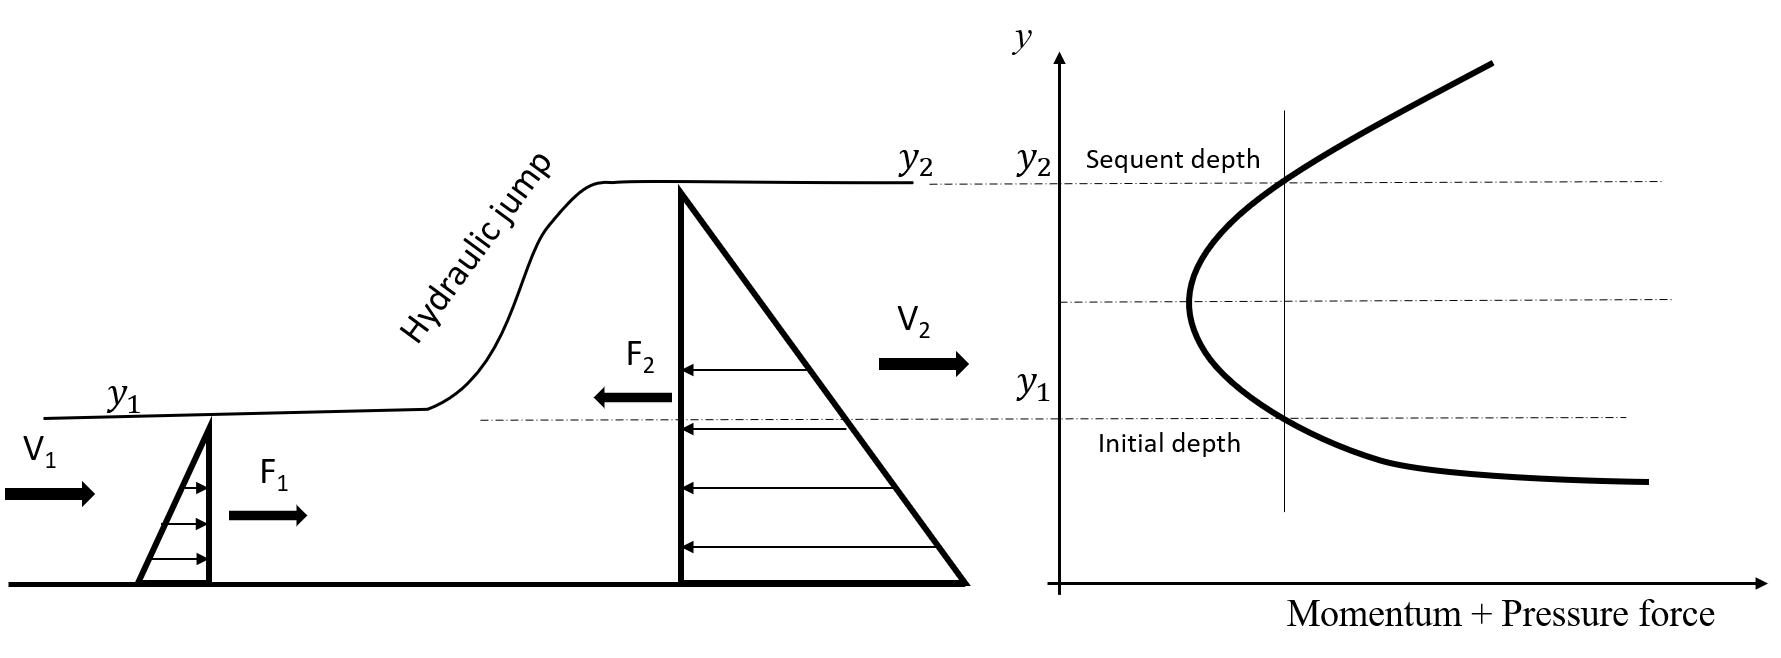
\includegraphics[scale=0.5]{./images/force_on_hydraulic_jump.png}
	\caption{Forces applied to the control volume containing the hydraulic jump}
	\label{fig:1112}
\end{figure}  

\begin{equation*}
\text{Resultant pressure force in } x-\text{direction} = P_1  - P_2
\end{equation*}
\begin{equation*}
\text{Rate of Momentum change } = M_2  - M_1
\end{equation*}
\begin{equation*}
 M_2  - M_1 = P_1  - P_2 
\end{equation*}

Or for a constant discharge
 \begin{equation*}
 M_2  - M_1 =  P_1  - P_2 = \text{constant}
 \end{equation*}
For a rectangular channel we can write these expressions (folowing section \ref{sec:force_on_struct} above) as
\begin{equation*}
\begin{aligned}[c]
P_1 & = \rho g \frac{y_1}{2}y_1b\\
M_1 &= \rho Q V_1\\
&= \rho Q \frac{Q}{y_1b}
\end{aligned}
\qquad\qquad
\begin{aligned}[c]
P_2 & = \rho g \frac{y_2}{2}y_2b\\
M_2 &= \rho Q V_2\\
&= \rho Q \frac{Q}{y_2b}
\end{aligned}
\end{equation*}

Substituting for these and rearranging gives
 \begin{equation}
y_2  = \frac{y_1}{2} \left(\sqrt{1+8F_{r1}^{2}}-1\right)
\label{eq:conj_y2_from_y1}
\end{equation}
Or
 \begin{equation}
y_1  = \frac{y_2}{2} \left(\sqrt{1+8F_{r2}^2}-1\right)
\label{eq:conj_y1_from_y2}
\end{equation}

Thus, knowing the discharge and either one of the depths on the upstream or downstream side of the jump, the other - or \textit{sequent} (or \textit{conjugate} or \textit{alternate}) depth - may be easily computed. 

More manipulation of  Equation \ref{eq:ycrit_esc} and the specific energy gives the energy loss in the jump as

 \begin{equation}
\Delta E  = \frac{(y_2-y_1)^3}{4y_1y_2} \left(\sqrt{1+8F_{r2}^2}-1\right)
\label{eq:deltaE}
\end{equation}
%Equation 1.23

These are useful results in particular for gradually varied flow calculations to determine water surface profiles enabling detection and positioning of hydraulic jumps.

In summary, for a hydraulic jump will only occur if the upstream flow is super-critical. The higher the upstream Froude number the higher the jump and the greater the loss of energy in the jump.

\subsection{Rapidly varied flow and Critical-depth structures}
The effect of a local rise in the bed level on the flow has been discussed earlier. It was shown that the depth would fall as the flow went over the rise. If this rise were large enough (for the particular velocity) the fall would be enough to give critical depth over the rise. Increasing the rise further would not decrease the depth but it would remain at critical depth. This observation may be confirmed by studying further the specific energy equation in a similar way to earlier.

The fact that depth is critical over the rise and that critical depth can be calculated quite easily for a give discharge is made use of in hydraulic structures for flow measurement. Actually it is the converse of the above, that the discharge can be easily calculated if the critical depth is known, that is most useful.

\subsubsection{Broad-crested weir}

\begin{figure}[H]
	\centering
	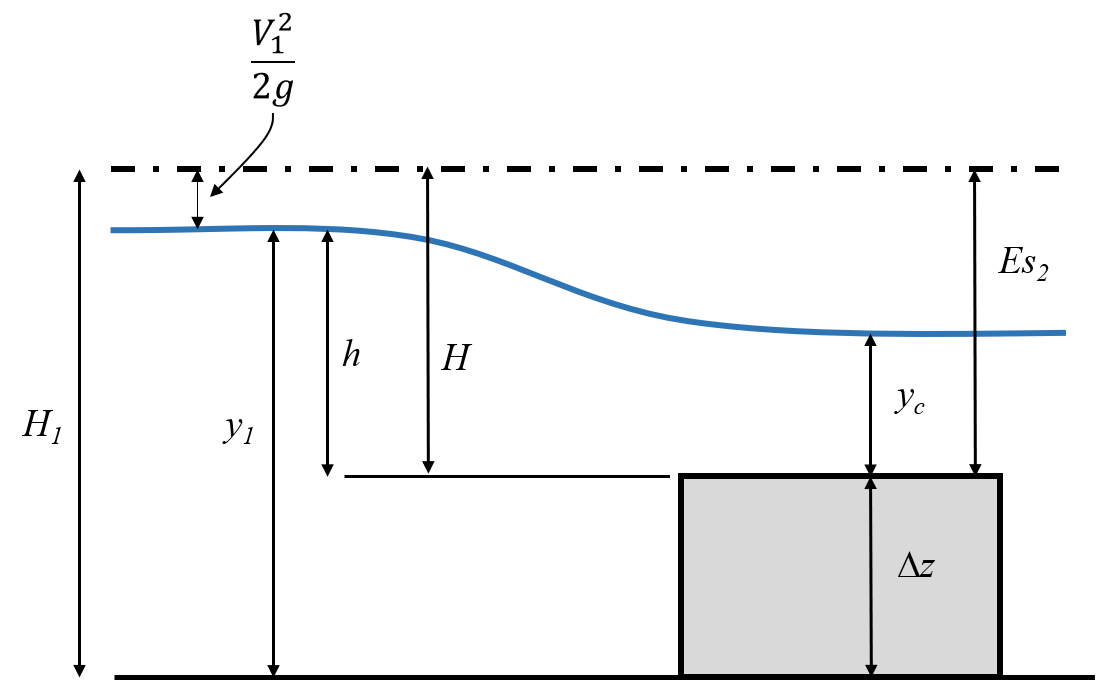
\includegraphics[scale=0.7]{./images/flow_over_broad_crested_weir.png}
	\caption{Flow over a broad crested weir}
	\label{fig:1181}
\end{figure} 

Assuming that the depth is critical over the rise then we know
\begin{equation*}
V_2 = V_c = \sqrt{gy_c}
\end{equation*} 
\begin{equation*}
Q = AV_c = by_c\sqrt{gy_c}
\end{equation*} 
where $b$ is the width of the channel

Earlier it was shown in Eqn \ref{eq:ycrit_esc} that 
\begin{equation*}
y_c = \frac{2}{3}E_{sc}
%\label{eq:ycrit_esc} % 1.19
\end{equation*} 

Assuming no energy loss between 1 and 2
\begin{align*}
E_{s_2} &= h + \frac{V_1^2}{2g} = H \\
y_c &= \frac{2}{3}H
\end{align*}
So
\begin{align*}
Q &= \frac{2}{3} \sqrt{\frac{2g}{3}}bh^{3/2} \\
&= 1.705 bh^{3/2}
\end{align*}
in practice there are energy losses upstream of the weir. To incorporate this a coefficient of discharge and of velocity are introduced to give
\begin{equation}
Q = C_d C_v 1.705 bh^{3/2}
\label{eq:broad_crested_wweir}
\end{equation}

\subsubsection{Flumes} 
A second method of measuring flow by causing critical depth is to contract the flow. Similar specific energy arguments to those used for a raised bed can be used in analysis of this situation, and they come to similar predictions that depth will fall and not fall below critical depth.

It is also possible to combine the two by putting a raised section within the narrowed section.

These types of structures are known as flume, and the first type is known as a Venturi flume.

\subsubsection{Venturi flume}

Flumes are usually designed to achieve critical depth in the narrowest section (the throat) while also giving a very small afflux.

\begin{figure}[H]
	\centering
	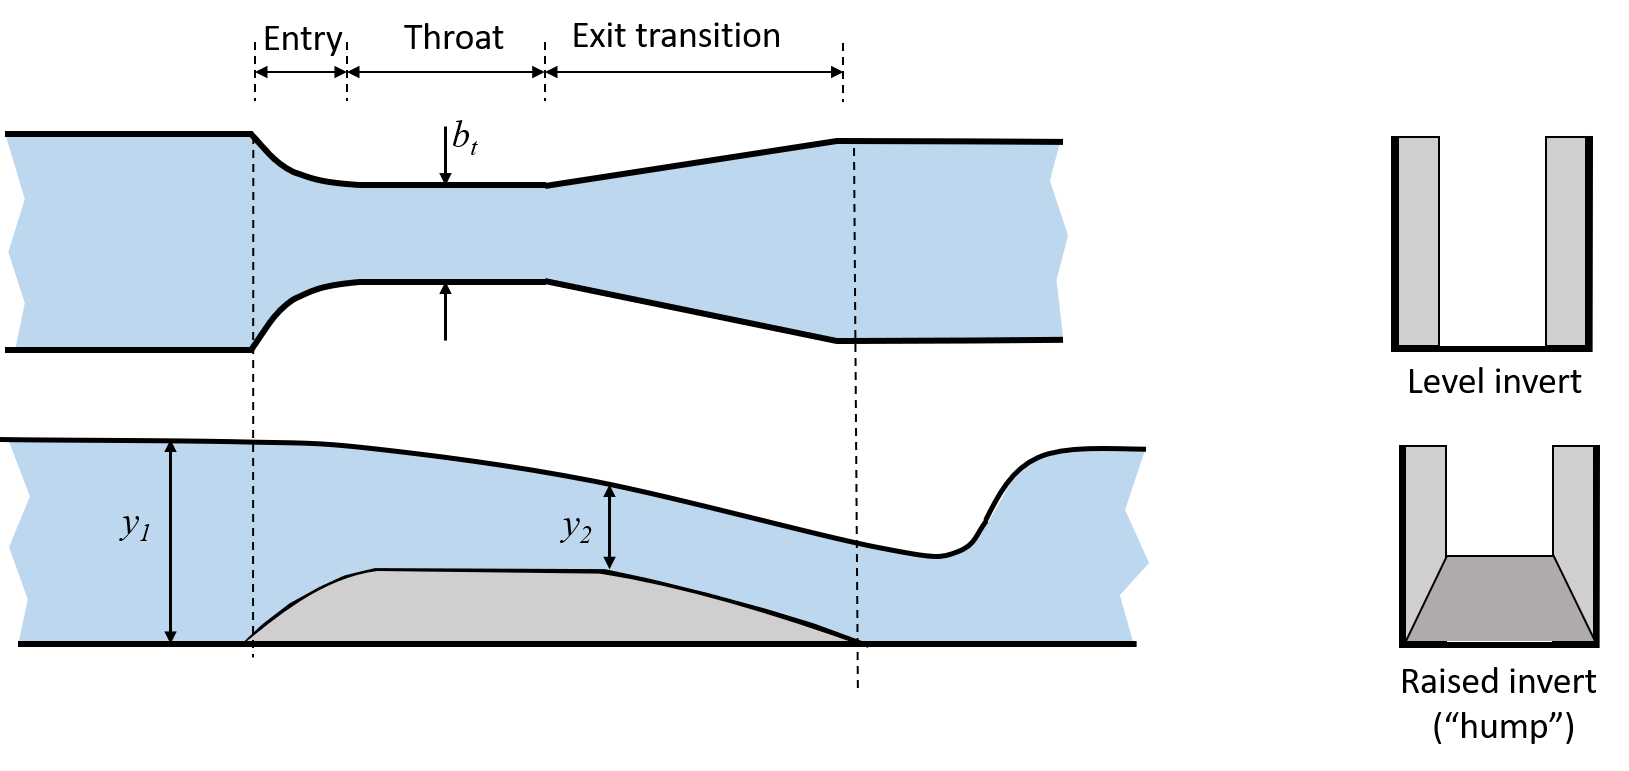
\includegraphics[scale=0.5]{./images/venturi_flume.png}
	\caption{Section through a Venturi flume}
	\label{fig:1191}
\end{figure}


The general equation for the ideal discharge through a flume can be obtained from the energy and continuity considerations.

The energy equation gives:
\begin{equation*}
E_s = y_1  + \frac{  V_1^2}{2g} = y_2  + \frac{  V_2^2}{2g} 
\end{equation*}

by continuity $V_1 = Q/(by_1) $ and $V_2 = Q/(b_2 y_2)$

which when substituted into the energy equation gives
\begin{equation*}
Q = b y_1 \sqrt{\frac{2g(y_1-y_2)}{[(b y_1) / (b_2 y_2)]^2 - 1}}
\end{equation*}


If critical flow is achieved in the throat then $y_2 = \frac{2}{3} E_s$ which can be substituted to give (in SI units)
\begin{equation*}
Q = 1.705 b_2 E_s^{3/2}
\end{equation*} 

or introducing a velocity correction factor and a discharge coefficient
\begin{equation}
Q = 1.705 b_2 C_v C_d y_1^{3/2}
\label{eq:venturi_flume}
\end{equation} 



\newpage
\section{Gradually varied flow}
\subsection{Channel Slope and Friction}
In the previous section of rapidly varied flow little mention was made of losses due to friction or the influence of the bed slope. It was assumed that frictional losses were insignificant - this is reasonable because rapidly varied flow occurs over a very short distance. However when it comes to long distances they become very important, and as gradually varied flow occurs over long distances we will consider friction losses here.

In the section on specific energy, \ref{sec:Es}, it was noted that there are two depth possible in uniform flow for a given discharge at any point in the channel. (One is super-critical the other sub-critical.) The solution of the Manning equation results in only one depth - the normal depth. 

It is the inclusion of the channel slope and friction that allow us to decide which of the two depths is correct. i.e. the channel slope and friction determine whether the uniform flow in the channel is sub or super-critical.

The procedure is 
\begin{enumerate}
	\item Calculate the normal depth from Manning's equation \ref{eq:manning_q}
	\item Calculate the critical depth from equation \ref{eq:crit_Q_general}
\end{enumerate}
The normal depth may be grewater, less than or equal to the critical depth. 
Comparing these enables us to identify whether we have sub or super-critical flow in the channel:
\begin{itemize}
	\item if the normal depth \textbf{greater than} critical depth then flow is \textbf{sub-critical}
	\item if the normal depth \textbf{less than} critical depth then flow is \textbf{super-critical}
\end{itemize}

An alternative way to view this is to examine the channel slope for a given roughness.

For a given channel and roughness there is only one slope that will give the normal depth equal to the critical depth. This slope is known as the critical slope ($S_c$).

If the slope is \textbf{less} than $S_c$ the normal depth will be \textbf{greater} than critical depth and the flow will be \textbf{sub-critical} flow. The slope is termed \underline{mild}.

If the slope is \textbf{greater} than $S_c$ the normal depth will be \textbf{less} than critical depth and the flow will be \textbf{super-critical} flow. The slope is termed \underline{steep}
.

\subsubsection{Transitions between sub and super critical flow}

If sub critical flow exists in a channel of a mild slope and this channel meets with a steep channel in which the normal depth is super-critical there must be some change of surface level between the two. In this situation the surface changes gradually between the two. The flow in the joining region is known as gradually varied flow.


This situation can be clearly seen in the figure on the left below. Note how at the point of joining of the two channels the depth passes through the critical depth.
%\begin{figure}[H]
%	\centering
%	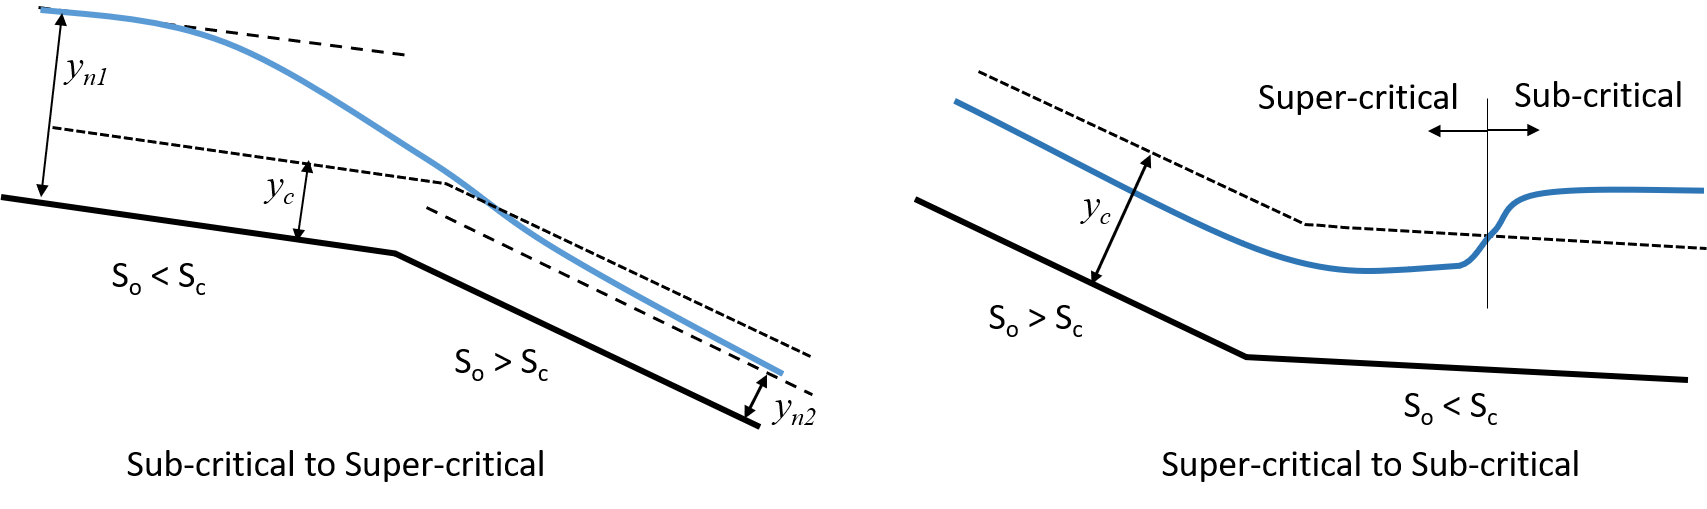
\includegraphics[width=0.8\textwidth]{./images/transition_sub_super_x2.png}
%	\caption{Transition from sup bo super-critical flow \cite{chadwick}}
%	\label{fig:1131}
%\end{figure} 
\begin{figure}[H]
  \centering
  \begin{subfigure}[b]{0.4\textwidth}
	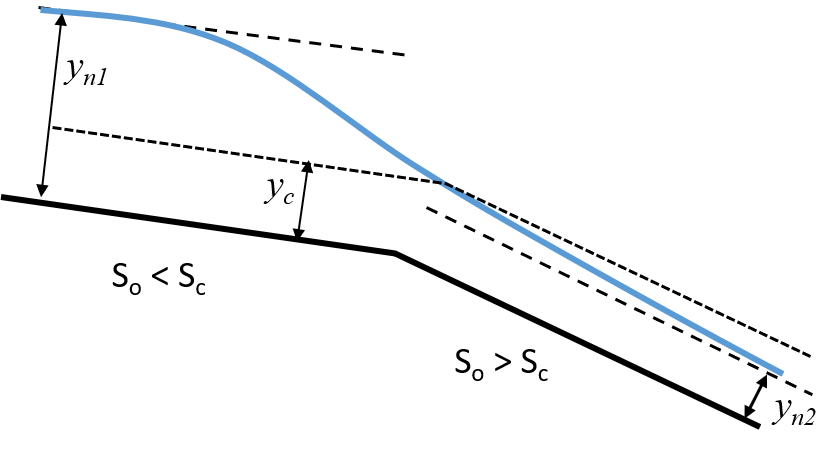
\includegraphics[width=\textwidth]{./images/transition_sub_super.png}
	\caption{Sub-critical to Super-critical}
	\label{fig:1131b}
  \end{subfigure}
%
  \begin{subfigure}[b]{0.4\textwidth}
	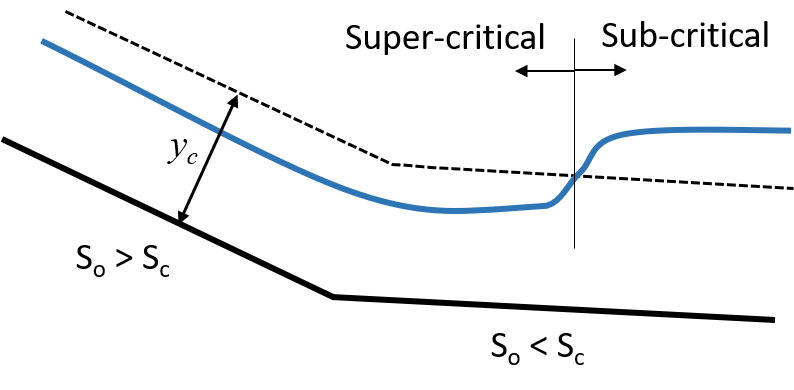
\includegraphics[width=\textwidth]{./images/transition_super_sub.png}
	\caption{Super-critical to Sub-critical}
	\label{fig:1131c}
  \end{subfigure}
  \caption{Transition from sub to super-critical flow}
  \label{fig:1131}
\end{figure}  
If the situation is reversed and the upstream slope is steep, super critical flow, and the down stream mild, sub-critical, then there must occur a hydraulic jump to join the two. There may occur a short length of gradually varied flow between the channel junction and the jump. The figure above right shows this situation:

Analysis of gradually varied flow can identify the type of profile for the transition as well as position hydraulic jumps.


\subsection{The equations of gradually varied flow}

The basic assumption in the derivation of this equation is the assumption that the change in energy with distance is equal to the friction loses.

\begin{equation}
\frac{dH}{dx} = -S_f
\label{eq:gvf_0}
\end{equation}
Taking the Bernoulli equation, eqn: \ref{eq:bernoulli_channel}, (repeated here):
  \begin{equation}
y  + \frac{ \alpha V^2}{2g} + z  = H
\label{eq:bernoulli_channel2}
\end{equation} 
and differentiating and equating to the friction slope
\begin{equation}
\frac{d}{dx}\left(y  + \frac{ \alpha V^2}{2g}\right) = - \frac{dz}{dx} -S_f
\end{equation}
or using the bed slope definition
\begin{equation}
S_o \left(=-\frac{dz}{dx}\right)
\end{equation}
\begin{equation}
\frac{dE_s}{dx} = S_o-S_f
\label{eq:gvf_1} % 1.25
\end{equation}

We saw earlier how specific energy changes with depth (derivation of Equation \ref{eq:crit_Q_general})
\begin{equation}
\frac{dE_s}{dx} = 1 - \frac{Q^2 B}{g A^3} = 1 - F_r^2
\label{eq:gvf_2} % 
\end{equation} 

Combining this with equation \ref{eq:gvf_1} gives
\begin{equation}
\frac{dy}{dx} = \frac{S_o-S_f}{1 - F_r^2}
\label{eq:gvf} % 1.26
\end{equation} 

This is the basic equation of gradually varied flow. It described how the depth, $y$, changes with distance $x$, in terms of the bed slope $S_o$, friction $S_f$ and the discharge, $Q$, and channels shape (encompassed in $F_r$).

Equations \ref{eq:gvf_1} and \ref{eq:gvf} are differential equations equating relating depth to distance. There is no explicit solution (except for a few special cases in prismatic channels). Numerical integration is the only practical method of solution. This is normally done on computers, however it is not too cumbersome to be done by hand.

\subsubsection{Friction slope, $S_f$, in gradually varied flow}
\label{sec:sf}
For the determination of the friction slope in gradually varied flow we make the assumption that energy loss is the as in \textit{uniforn flow}. 
Recall that in uniform flow the friction slope is equal to the bed slope i.e. $S_o = S_f$.

In uniform flow we have the Chezy (\ref{eq:chezy_v}) or Manning's (\ref{eq:manning_v}) equations, which written in terms of $V$ with the friction slope equated to the bed slope are:
\begin{equation*}
V = C\sqrt{R S_f}
\label{eq:chezy_v_sf}
\end{equation*} 
and
\begin{equation*}
V = \frac{1}{n}R^{2/3}S_f^{1/2}
\label{eq:manning_v_sf}
\end{equation*} 
Rearranging these gives expressions we can use for $S_f$ in gradually varied flow:
\begin{equation}
S_f = \frac{V^2}{C^2R}
\label{eq:sf_chezy_v}
\end{equation}
or
\begin{equation}
S_f = \frac{n^2V^2}{R^{4/3}}
\label{eq:sf_manning_v}
\end{equation}
or, in terms of $Q$
\begin{equation}
S_f = \frac{n^2Q^2}{R^{4/3}A^2}
\label{eq:sf_manning_q}
\end{equation}

\subsubsection{Critical Slope, $S_c$, evaluation}

We have the Manning's equation \ref{eq:manning_q} that gives normal depth 
\begin{equation*}
Q = \frac{1}{n}\frac{A^{5/3}}{P^{2/3}}S_o^{1/2}
%\label{eq:manning_q} %eq 1.11
\end{equation*} 

and equation \ref{eq:crit_Q_general} for $F_r$  at critical depth (taking $\alpha = 1$)
\begin{equation*}
\frac{Q^2 B_c}{gA_c^{3}} = 1
%\label{eq:crit_Q_general} % eq 1.17
\end{equation*}


Rearranging these in terms of Q and equating gives:
\begin{equation}
\frac{1}n{}\frac{A_c^{5/3}}{P_c^{2/3}}S_c^{1/2} = \sqrt{\frac{g A_c^3}{B_c}}
\end{equation} 

\begin{equation}
S_c = \frac{gn^2P_c}{B_c R_c^{1/3}}
\label{eq:sc}
\end{equation} 

(Note that the $c$ subscript indicates that these parameters are all at critical depth.)

\textbf{Critical Slope for a Wide Channel}

For the simple case of a \textit{wide} rectangular channel, width $B = b$, $A = by$ and $P\approx b$, then the above equation becomes
\begin{equation}
S_c = \frac{gn^2}{y_c^{1/3}}
\label{eq:sc_wide} % 1.24
\end{equation}

Note that this equation is \textit{explicit} in either $S_c$ or $y_c$, so are straightforward to calculated.


\subsection{Classification of profiles}

Before attempting to solve the gradually varied flow equation a great deal of insight into the type of solutions and profiles possible can be gained by taking some time to examine the equation. Time spent over this is almost compulsory if you are to understand steady flow in open channels.

For a given discharge, $S_f$ and $F_r^2$ are functions of depth. 
\begin{equation}
S_f = \frac{n^2 Q^2}{R^{4/3}A^2} 
\label{eq:sf1} 
\end{equation} 
\begin{equation}
F_r^2 = \frac{Q^2 B}{gA^3} 
\label{eq:fr3} 
\end{equation} 
A quick examination of these two expressions shows that they both increase with $A$, i.e. increase with $y$.

We also know that when we have \textbf{uniform} flow
\begin{equation*}
S_f =  S_o	\qquad	\text{and} \qquad 	y = y_n
\end{equation*}
 So
\begin{equation*}
 S_f > S_o	\qquad	\text{when} \qquad 	y < y_n
\end{equation*}		
\begin{equation*}
S_f < S_o	\qquad	\text{when} \qquad 	y > y_n
\end{equation*}
and
\begin{equation*}
F_r^2 > 1	\qquad	\text{when} \qquad 	y < y_c
\end{equation*}
\begin{equation*}
F_r^2 < 1	\qquad	\text{when} \qquad 	y > y_c
\end{equation*}
From these inequalities we can see how the sign of $dy/dx$ i.e. the surface slope changes for different slopes and Froude numbers.

Taking the example of a \textbf{mild} slope, shown in the figure \ref{fig:1151b} below:
%    \begin{figure}[H]
% 	\centering
% 	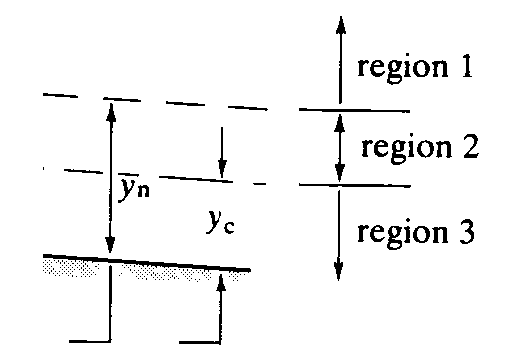
\includegraphics[scale=0.6]{./images/fig_1151.png}
% 	\caption{Flow zones / regions (for a mild slope) \cite{chadwick}}
% 	\label{fig:1151a}
% \end{figure}  
\begin{figure}[H]
	\centering
	\begin{subfigure}[b]{0.4\textwidth}
		\centering
		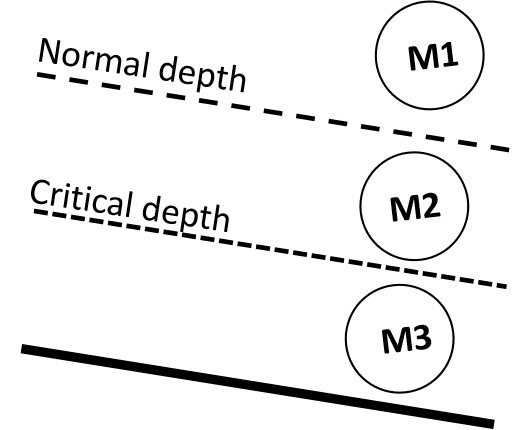
\includegraphics[scale=0.5]{./images/mild_slope_regions.png}
		\caption{Flow region lables for \textbf{mild slope}}
		\label{fig:1151b}
	\end{subfigure}
	\qquad \qquad
	\begin{subfigure}[b]{0.4\textwidth}
		\centering
		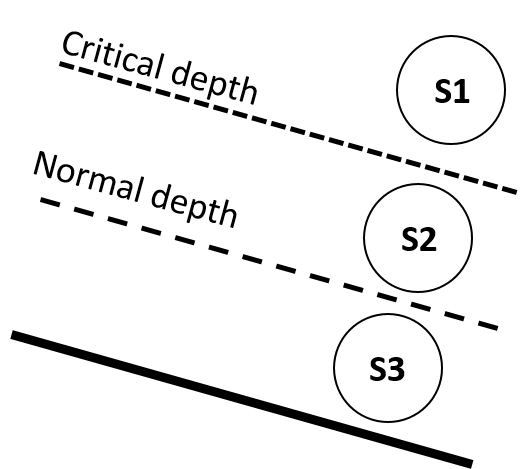
\includegraphics[scale=0.5]{./images/steep_slope_regions.png}
		\caption{Flow region lables for \textbf{steep slope}}
		\label{fig:1151c}
	\end{subfigure}
	\caption{Flow region lables for mild and steep slopes}
	\label{fig:1151}
\end{figure} 
The normal and critical depths are shown (as it is mild, normal depth is greater than critical depth). Treating the flow as to be in three zones: 
\begin{itemize}
	\item zone 1, above the normal depth. Here will be $M1$ surface profile. 
\item zone 2, between normal and critical depth. Here will be $M2$ surface profile. 
\item zone 3, below critical depth. Here will be  $M3$ surface profile. 
\end{itemize}
The direction of the surface inclination may thus be determined for each zone. Remembering equation \ref{eq:gvf}
\begin{equation*}
\frac{dy}{dx} = \frac{S_o-S_f}{1 - F_r^2}
\label{eq:gvf_v2} % 1.26
\end{equation*} 

\textbf{zone 1}
\begin{equation*}
y > y_n > y_c		\qquad	Sf < So		\qquad	F_r^2 < 1	\qquad \Rightarrow	\qquad	dy/dx \text{ is positive, surface rising}
\end{equation*}

\textbf{zone 2}
\begin{equation*}
y_n > y > y_c	\qquad	S_f > S_o	\qquad	F_r^2 < 1		\qquad \Rightarrow	\qquad		dy/dx \text{ is negative, surface falling}
\end{equation*}

\textbf{zone 3}
\begin{equation*}
y_n > y_c > y	\qquad	S_f > S_o	\qquad	F_r^2 > 1		\qquad \Rightarrow	\qquad		dy/dx \text{ is positive,surface rising
}
\end{equation*}

The condition at the boundary of the gradually varied flow may also be determined in a similar manner:

\textbf{zone 1}
\begin{equation*}
\text{As } y \rightarrow \infty \text{ then } S_f \text{ and } F_r \rightarrow 0 \text{ and } dy/dx \rightarrow S_o
\end{equation*}
Hence the water surface is asymptotic to a horizontal line for it maximum
\begin{equation*}
\text{As } y \rightarrow y_n \text{ then } S_f \rightarrow S_o \text{ and } dy/dx \rightarrow 0
\end{equation*}
Hence the water surface is asymptotic to the line $y = y_n$

\textbf{zone 2}
As for zone 1 as $y$ approaches  normal depth:
\begin{equation*}
\text{As } y \rightarrow y_n \text{ then } S_f \rightarrow S_o \text{ and } dy/dx \rightarrow 0
\end{equation*}
Hence the water surface is asymptotic to the line $y = y_n$

But a problem occurs when $y$ approaches the critical depth:
\begin{equation*}
\text{As } y \rightarrow y_c \text{ then } F_r \rightarrow 1 \text{ and } dy/dx \rightarrow \infty
\end{equation*}
This is physically impossible but may be explained by the pointing out that in this region the gradually varied flow equation is not applicable because at this point the fluid is in the rapidly varied flow regime.
In reality a very steep surface will occur (and possibly a hydraulic jump).

\textbf{zone 3}
As for zone 2 a problem occurs when $y$ approaches the critical depth:
\begin{equation*}
\text{As } y \rightarrow y_c \text{ then } F_r \rightarrow 1 \text{ and } dy/dx \rightarrow \infty
\end{equation*}
Again we have the same physical impossibility with the same explanation.
And again in reality a very steep surface will occur.

\begin{equation*}
\text{As } y \rightarrow 0 \text{ then } dy/dx \rightarrow S_o \text{ the slope of bed of the channel}
\end{equation*}

The gradually varied flow equation is not valid here but it is clear what occurs (the channel is dry!).

\newpage
In general (and key to remember), 
\begin{itemize}
	\item normal depth is approached \underline{asymptotically} 
	\item critical depth at \underline{right angles}
\end{itemize}.

The possible surface profiles within each zone can be drawn from the above considerations. These are shown for the mild sloped channel below.
\begin{figure}[H]
	\centering
	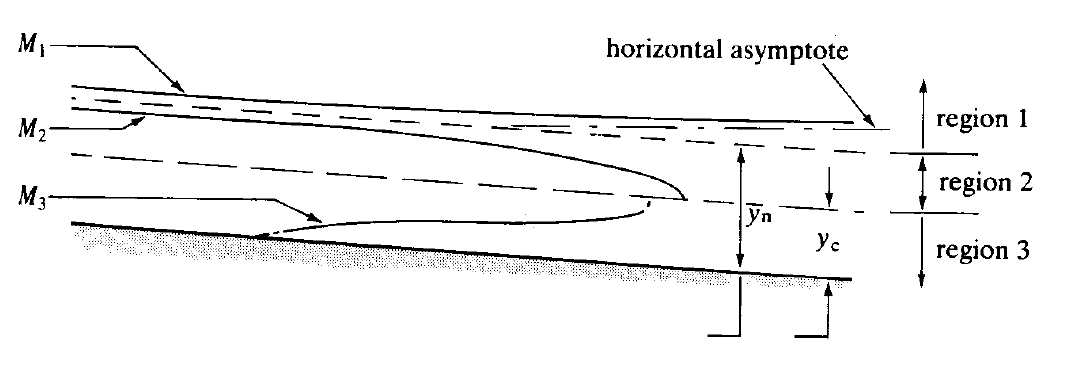
\includegraphics[scale=0.6,angle=1]{./images/fig_1152.png}
	\caption{The gradually varied flow surface profiles in a mild sloped channel, \cite{chadwick}}
	\label{fig:1152}
\end{figure}  
The surface profile in zone 1 of a mild slope is called an M1 curve, in zone 2 an M2 curve and in zone 3 an M3 curve.

All the possible surface profiles for all possible slopes of channel (there are 15 possibilities) are shown in the figure \ref{fig:1153} on the next page.
 

    \begin{figure}[p]
	\centering
	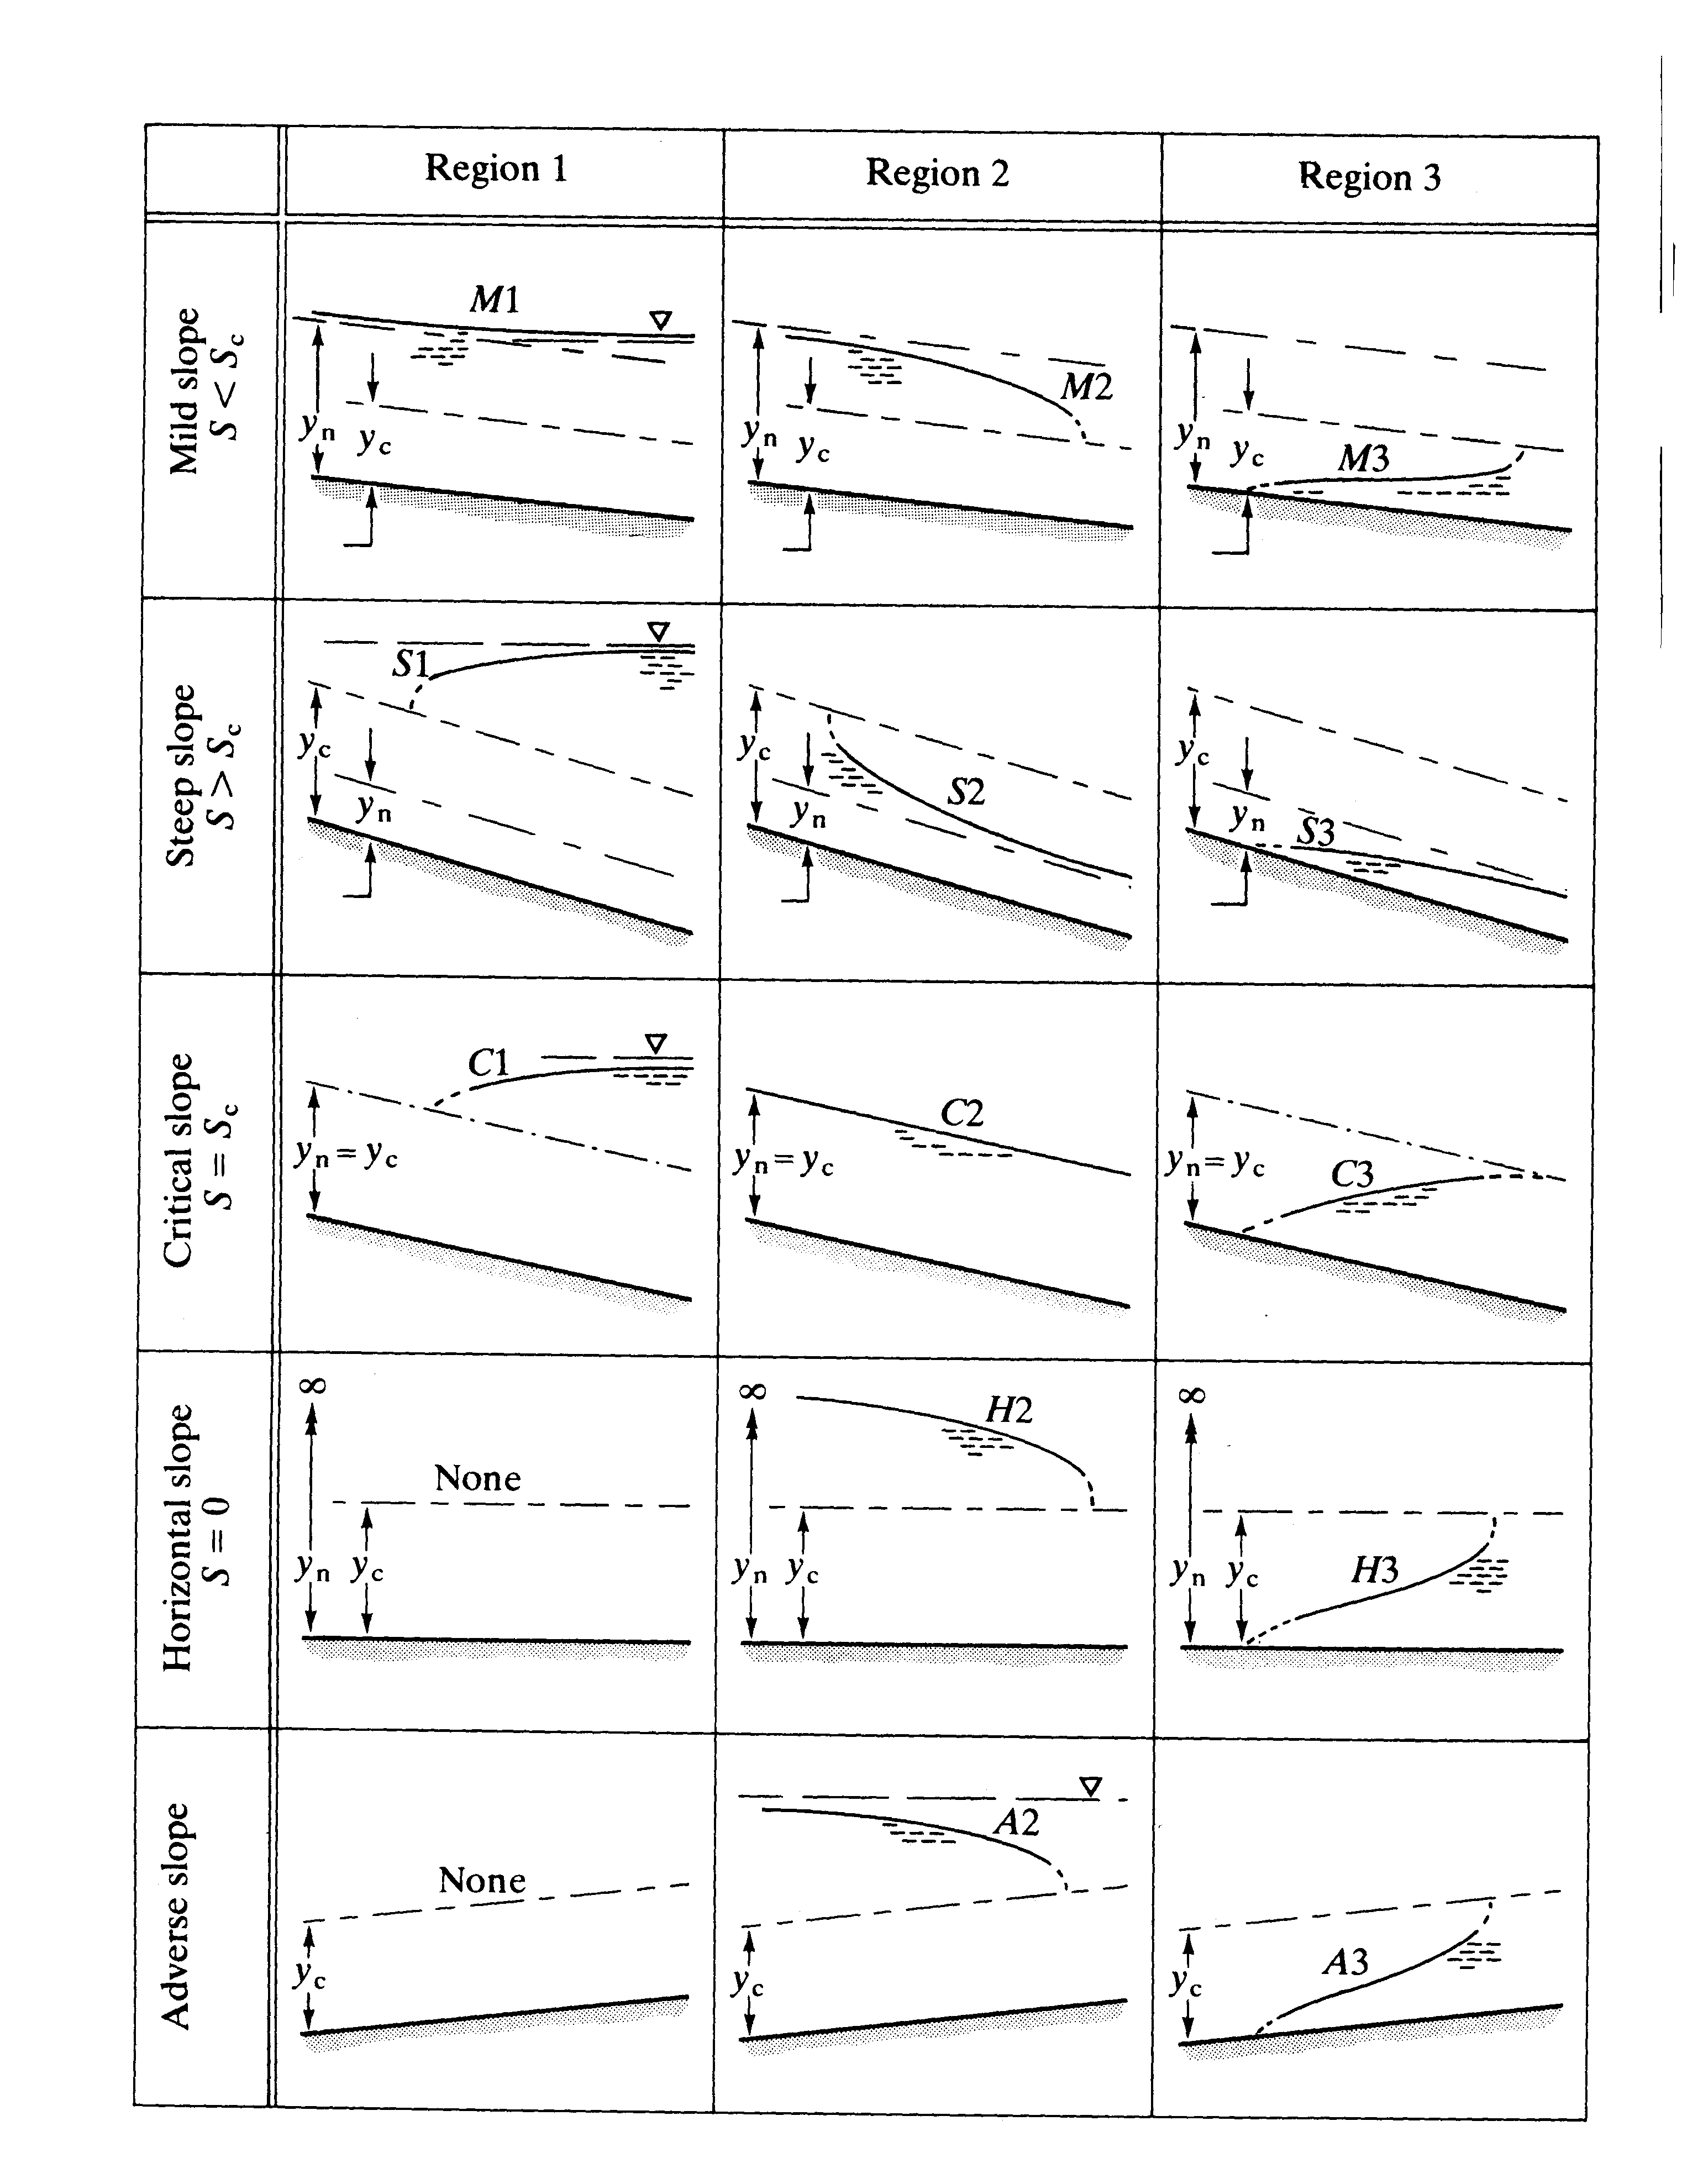
\includegraphics[scale=0.2,angle=0.5]{./images/fig_1153.png}
	\caption{The possible gradually varied flow profiles, \cite{chadwick}}
	\label{fig:1153}
\end{figure}   
 
\subsection{How to determine the surface profiles}

Before one of the profiles discussed above can be decided upon two things must be determined for the channel and flow:
\begin{enumerate}[label=\alph*]
	\item Whether the slope is mild, critical or steep. The normal and critical depths must be calculated for the design discharge
\item The positions of any control points must be established. Control points are points of known depth or relationship between depth and discharge. Example are weirs, flumes, gates or points where it is known critical flow occurs like at free outfalls, or that the flow is normal depth at some far distance down stream.
\end{enumerate}

Once these control points and depth position has been established the surface profiles can be drawn to join the control points with the insertion of hydraulic jumps where it is necessary to join sub and super critical flows that don't meet at a critical depth.

Below are two examples.
    \begin{figure}[H]
	\centering
	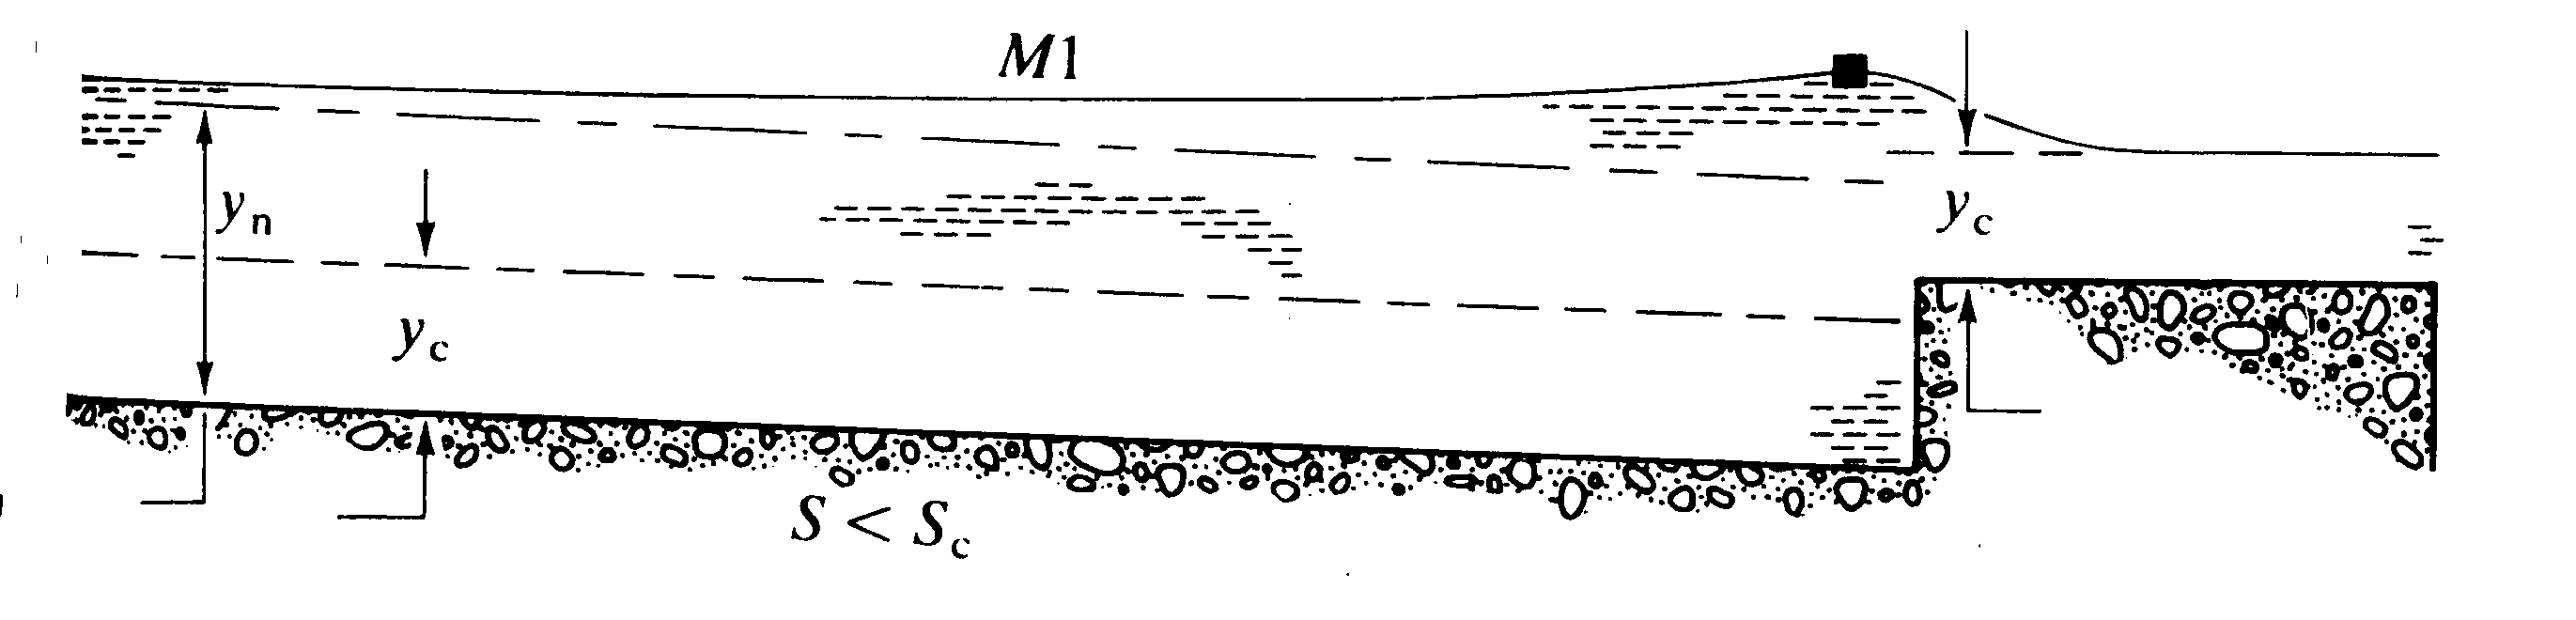
\includegraphics[scale=0.24]{./images/fig_1161.png}
	\caption{An example surface profile due to a broad crested weir, \cite{chadwick}}
	\label{fig:1161}
\end{figure}


This shows the control point just upstream of a broad crested weir in a channel of mild slope. The resulting curve is an M1.

    \begin{figure}[H]
	\centering
	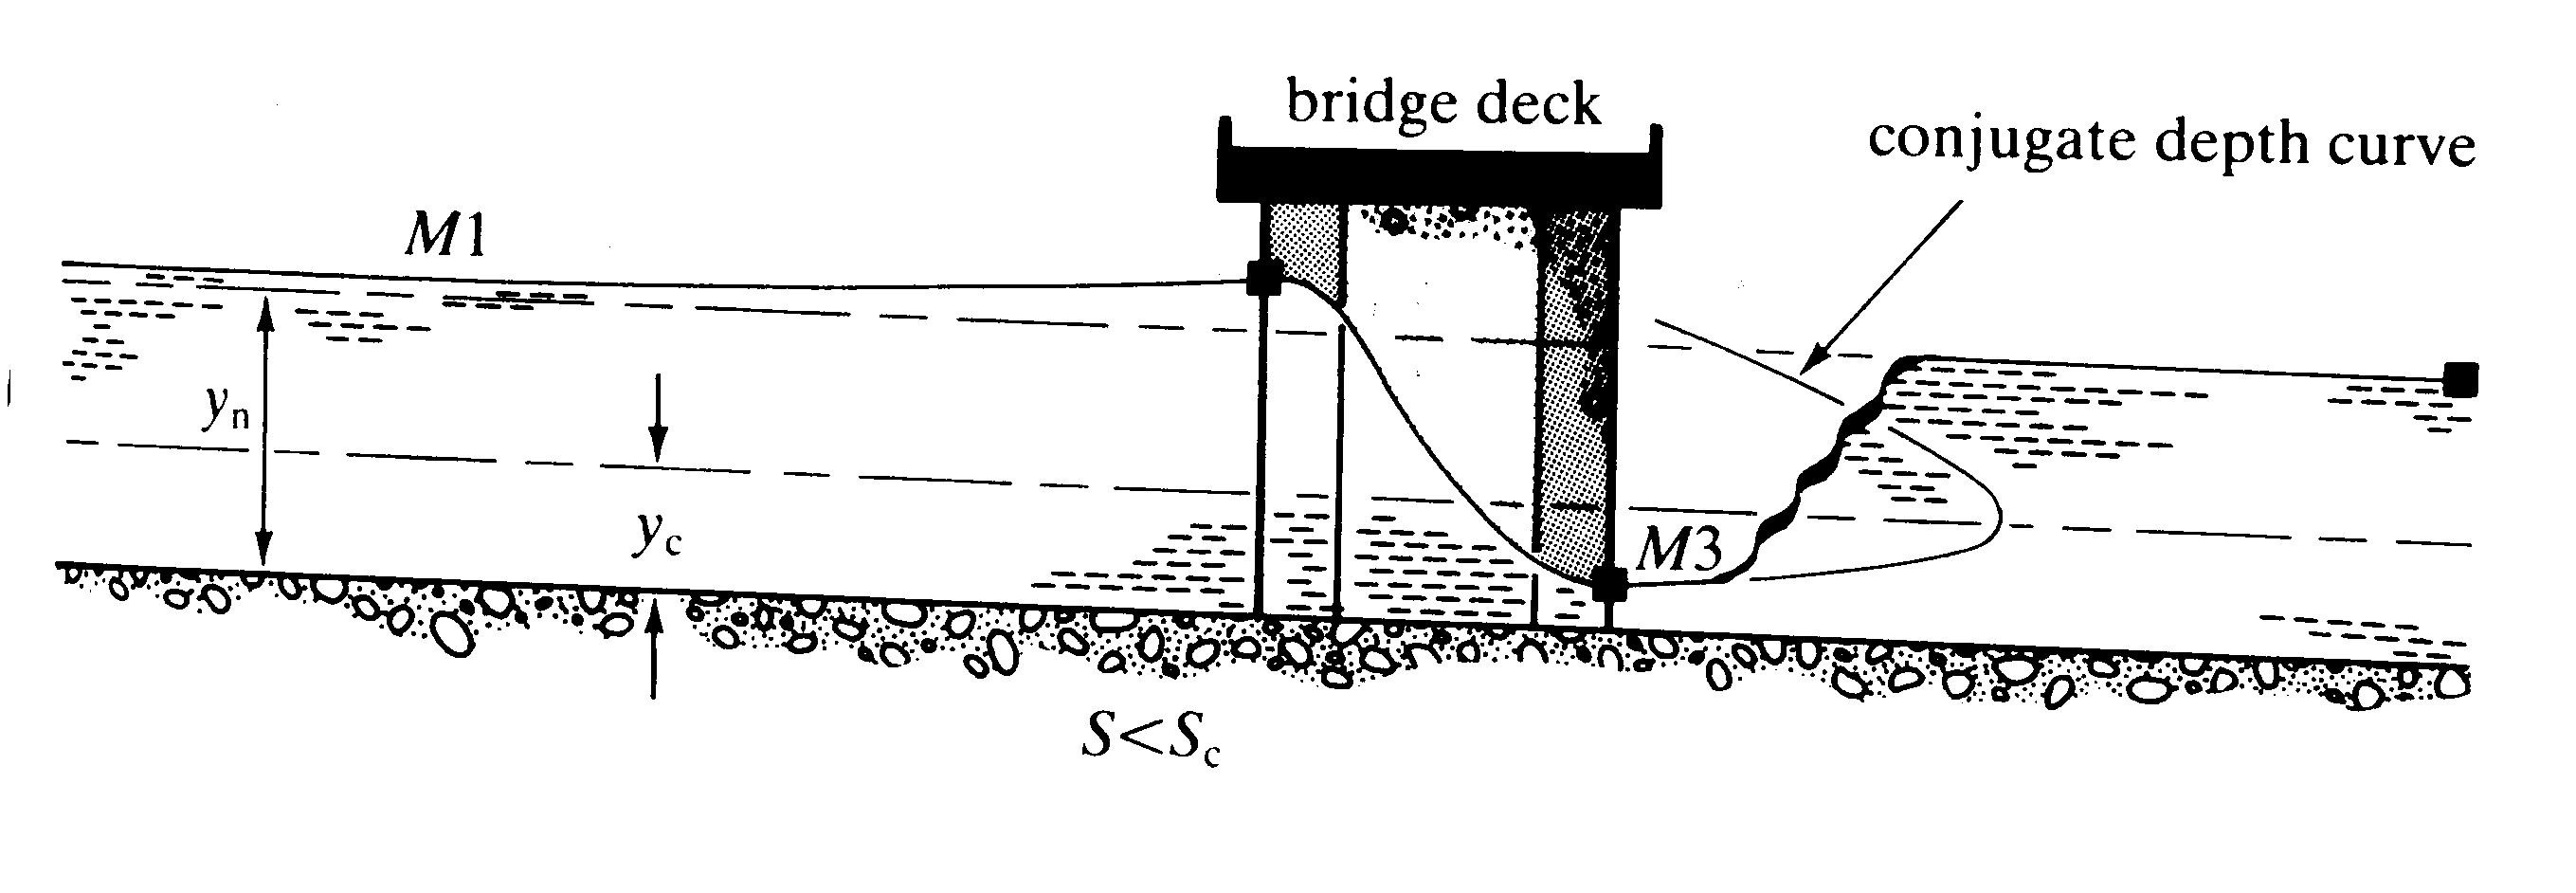
\includegraphics[scale=0.24]{./images/fig_1162.png}
	\caption{An example surface profile through a bridge when in flood, \cite{chadwick}}
	\label{fig:1162}
\end{figure} 


This shows how a bridge may act as a control - particularly under flood conditions. Upstream there is an M1 curve then flow through the bridge is rapidly varied and the depth drops below critical depth so on exit is super critical so a short M3 curve occurs before a hydraulic jump takes the depth back to a sub-critical level.

\newpage
\subsection{Method of solution of the Gradually varied flow equation}

There are three (equivalent) forms of the equations for gradually varied flow: Eqs \ref{eq:gvf_0}, \ref{eq:gvf_1} and \ref{eq:gvf}, which are respectively: 
\begin{equation*}
\frac{dH}{dx} = -S_f
%\label{eq:gvf_0}
\end{equation*}

\begin{equation*}
\frac{dE_s}{dx} = S_o-S_f
%\label{eq:gvf_1} % 1.25
\end{equation*}

\begin{equation*}
\frac{dy}{dx} = \frac{S_o-S_f}{1 - F_r^2}
%\label{eq:gvf} % 1.26
\end{equation*}  

In the past direct and graphical solution method have been used to solve these, however these method have been superseded by numerical methods which should now be the only method used.

\subsubsection{Numerical methods}

All (15) of the gradually varied flow profiles shown above may be quickly solved by simple numerical techniques. One computer program (or spreadsheet) can be written to solve most situations.

There are three basic numerical method that can be used 

\begin{enumerate}[label=\roman*,noitemsep]
	\item Direct step - distance from depth 
\item Standard step method - depth from distance
\item Numerical Integration (e.g. Euler's method) - which can give either distance from depth or depth from distance
\end{enumerate}

In each of these we will need to calculate $S_f$, sec section \ref{sec:sf}, that is calculated from the uniform flow equations to give, from Chezy eqn \ref{eq:sf_chezy_v} or from Manning's equation  \ref{eq:sf_manning_q}), i.e.:
\begin{equation}
S_f = S_o = \left( \frac{Q}{ACR^{1/2}}\right)^2 =\left( \frac{Q n}{A R^{2/3}}\right)^2 
\label{eq:sf}
\end{equation}

\subsubsection{The direct step method - distance from depth}
This method will calculate (by integrating the gradually varied flow equation) a distance for a given change in surface height.

The equation used is eqn. \ref{eq:gvf}, which written in finite difference form is
\begin{equation}
\Delta x = \Delta y \left(\frac{1 - F_r^2}{S_o-S_f}\right)_\text{mean}
\label{eq:gvf_direct_step} % 1.29
\end{equation}

\newpage 
The steps in solution are:
\begin{enumerate}[noitemsep]
	\item 	Determine the control depth as the starting point
\item 	Decide on the expected curve and depth change if possible
\item 	Choose a suitable depth step $\Delta y$
\item 	Calculate the term in brackets at the \textit{mean} depth between the current (initial) depth and depth at the next step  (i.e. $y_\text{mean} = y_\text{initial} + \Delta y/2$)
\item 	Calculate $\Delta x$
\item 	Repeat 4 and 5 until the appropriate distance / depth changed has been reached
\end{enumerate}
This is really best seen demonstrated in an example.

\subsubsection{The standard step method - depth from distance} 

This method will calculate (by integrating the gradually varied flow equation) a depth at a given distance up or downstream.

The equation used is \ref{eq:gvf_1}, which written in finite difference form is

\begin{equation}
\Delta E_s = \Delta x (S_o-S_f)_\text{mean}
\label{eq:gvf_standard_step} % 1.30
\end{equation} 


The steps in solution are similar to the direct step method shown above but for each $\Delta x$ there is the following iterative procedure:
\begin{enumerate}[noitemsep]
\item	Assume a value of depth $y$ (the control depth or the last solution depth)
\item	Calculate the specific energy $E_{s_x}$
\item	Calculate $S_f$
\item	Calculate $\Delta E_s$ using equation \ref{eq:gvf_standard_step}
\item	Calculate $E_{s_{(x+\Delta x)}} = E_{s_x} + \Delta E_s$
\item	Repeat until $E_{s_{(x+\Delta x)}}  = E_{s_x}$
\end{enumerate}

Again this is really best understood demonstrated in an example.

\subsubsection{The Standard step method - alternative form}

This method will again calculate a depth at a given distance up or downstream but this time the equation used is \ref{eq:gvf_0}, which written in finite difference form is
\begin{equation*}
\Delta H = \Delta x (S_f)_\text{mean}
\label{eq:gvf_0_discrete} % 1.31
\end{equation*}
Where $H$ is given by equation \ref{eq:bernoulli_channel}
  \begin{equation}
y  + \frac{ \alpha V^2}{2g} + z  = H
%\label{eq:bernoulli_channel} %1.14
\end{equation}
 
The strategy is the same as the first standard step method, with the same necessity to iterate for each step.

\subsubsection{Numerical Integration (Euler method)}
With computers and spreadsheets being common place, it is easy to setup a simple program or spreadsheet formulae to numerically integrate the gradually varied flow equations and to take a large number of steps very quickly. The advantage of this is that it enables very small length, $\Delta x$, or depth $\Delta y$ steps to be taken. This means that a low order integration method - such as the 1st order Euler method - may be used and sufficient accuracy optianed using the small steps to ensure reduced error.

The two formula below are equivalent to the Euler method stepping in depth or time. The subscript 'o' indicates that the function, i.e. the bracketed term, is calculated at the \textit{initial} or \textit{known} point. No itteration is required.
\begin{equation}
\Delta x = \Delta y \left(\frac{1-F_r^2}{S_o - S_f}\right)_0 \\
\end{equation}
or
\begin{equation}
\Delta y = \Delta x \left(\frac{S_o - S_f}{1-F_r^2}\right)_0 \\
\end{equation}


%\newpage
%\section{Examples}

\newpage
\appendix
\addcontentsline{toc}{section}{Appendices}
\section*{Appendices}
\section{Various formulations of the Uniform Flow Equations}
	This appendix demonstrates some of the various formulations of the equations of uniform-flow in an open-channel.
	
	There are a lot of equations in this document. Only the first 4 should be committed to memory. All of the others are derived from these 4 and you should become confident that you follow how they are obtained.
	\begin{figure}[H]
		\centering
		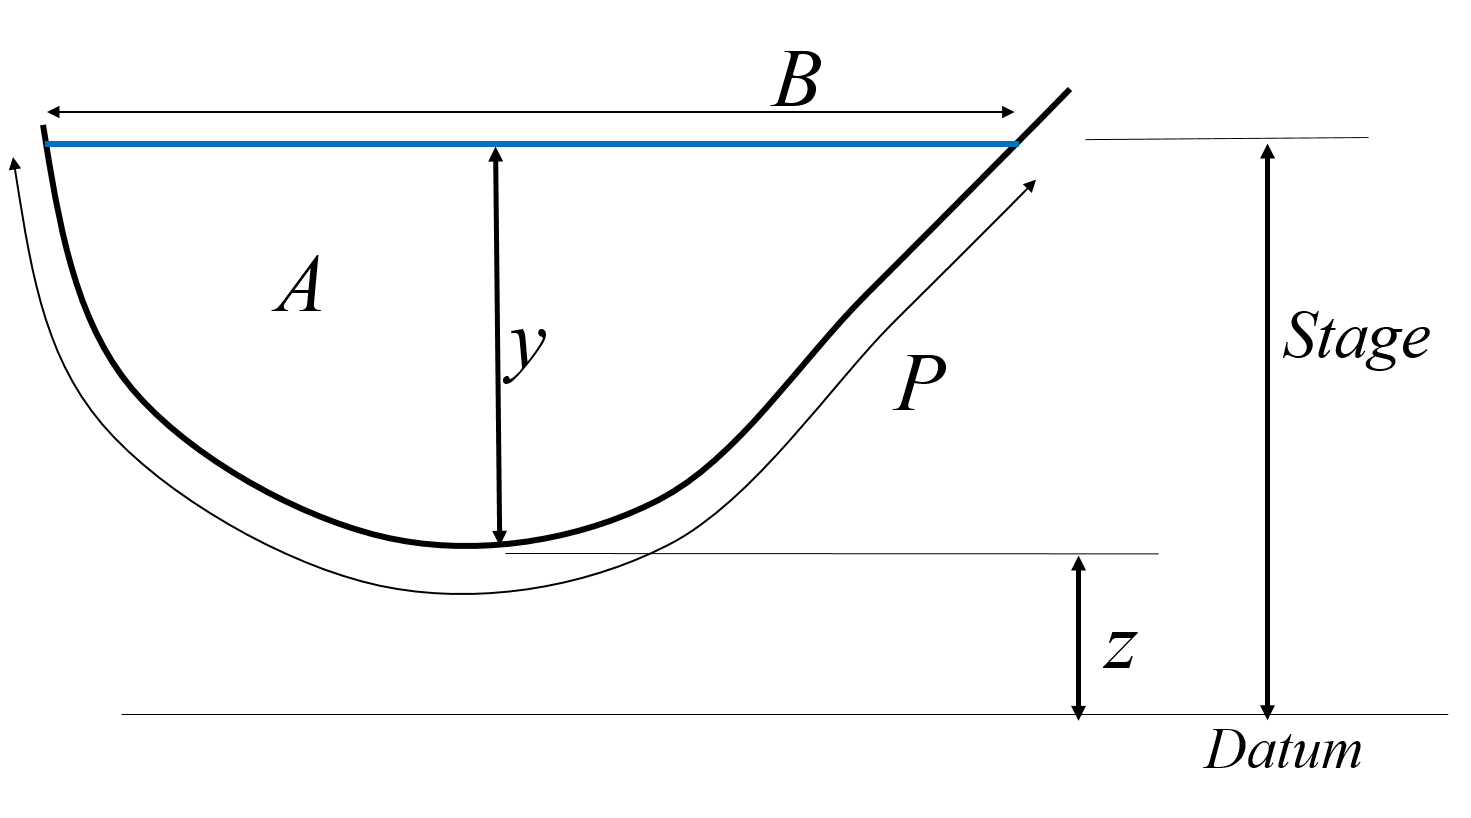
\includegraphics[width=10cm]{./images/section_general.png}
		\caption{A general section of a channel with notation}
		\label{fig:section_general}
	\end{figure}
	The equations take the basic parameters $Q =$ flow (discharge), $V = $ velocity, $y =$ depth, $A =$ cross-sectional Area, $B =$ surface width, $P =$ wetted perimeter and $S_o =$ bed slope.
	
	\subsection*{The Uniform Flow Equations}
	
	\subsubsection*{The Chezy Equation}
	The fundamental equation is the \textit{Chezy} equation where $C$ is the "Chezy $C$":
	\begin{align}
	V &= C\sqrt{RS_o} \nonumber \\
	&= CR^{1/2}S_o^{1/2}
	\label{eqn:chezyv}
	\end{align}
	
	And in terms of flow (discharge)
	\begin{align}
	Q &= A C \sqrt{RS_o}  \nonumber \\
	&= ACR^{1/2}S_o^{1/2}
	\label{eqn:chezy}
	\end{align}
	
	\subsubsection*{The Manning's equation}
	The Chezy $C$ and Manning's $n$ are related by:
	\begin{equation}
	C = \frac{R^{1/6}}{n} 
	\label{eqn:chezyn}
	\end{equation}
	
	So equation \ref{eqn:chezy} becomes
	
	\begin{align}
	Q &= \frac{1}{n}AR^{1/6}\sqrt{RS_o} \nonumber \\
	&= \frac{1}{n}AR^{2/3}S_o^{1/2}
	\label{eqn:manning}
	\end{align}
	
	\subsubsection*{In terms of $A$ and $P$}
	\textbf{Chezy} : substituting for $R = \frac{A}{P}$ Equation \ref{eqn:chezy} becomes
	\begin{align}
	Q &= A C \sqrt{\frac{AS_o}{P}}  \nonumber \\
	&= AC{\frac{A}{P}}^{1/2}S_o^{1/2} \nonumber \\
	&= C \frac{A^{3/2}}{P^{1/2}} S_o^{1/2} \nonumber \\
	&= CA^{3/2}{P}^{-1/2} S_o^{1/2} 
	\label{eqn:chezy_ap}
	\end{align}
	
	\textbf{Manning} : substituting for $R = \frac{A}{P}$ Equation \ref{eqn:manning} becomes
	
	\begin{align}
	Q &= \frac{1}{n}A \left( \frac{A}{P} \right)^{1/6} \sqrt{\frac{A}{P}S_o} \nonumber \\
	&= \frac{1}{n}A\left(\frac{A}{P}\right)^{2/3}S_o^{1/2} \nonumber \\
	&= \frac{1}{n}\frac{A^{5/3}}{P^{2/3}}S_o^{1/2} \nonumber \\
	&= \frac{1}{n} A^{5/3} P^{-2/3} S_o^{1/2} 
	%\label{eqn:manning_ap}
	\end{align}
	
	
	\subsection*{Channels of Common Geometry}
	There are a few cross-sections that are very commonly constructed i.e. rectangular, trapezoidal and circular. You should be familiar with the development of the equation of uniform flow for these. Do not rely on remembering them, it is much easier to derive them from the Chezy (\ref{eqn:chezy}) or Manning (\ref{eqn:manning}) generic equations.
	
	These equations are expressions in term of depth of flow $y_n$. This depth is refered to as the \textit{normal depth}.  \textbf{Do remember} that the depth of flow in a uniform flow equation is \textit{normal} depth - it is the depth that a long channel would naturally reach as gravitational and frictional forces balance.
	
	\subsubsection*{Rectangular Channels}
	\begin{figure}[H]
		\centering
		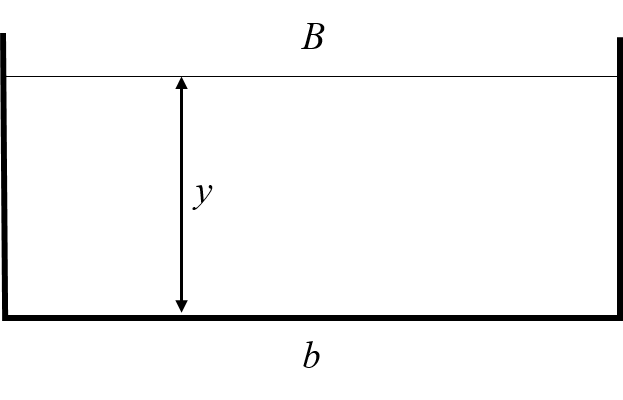
\includegraphics[width=7cm]{./images/section_rectangular.png}
		\caption{A rectangular channel section}
		\label{fig:section_rect}
	\end{figure}
	For a rectangular channel we have:
	\[ 
	A = by
	\] 
	and 
	\[
	P = b+2y
	\]
	so
	\[
	R = \frac{A}{P} = \frac{by}{b+2y}
	\]
	
	The Chezy equation, eqn \ref{eqn:chezy} for a rectangular channel becomes:
	\begin{equation}
	Q = C by_n \left( \frac{by_n}{b+2y_n}\right)^{1/2}S_o^{1/2}
	\label{eqn:chezy_sq}
	\end{equation}
	
	The Manning equation, eqn \ref{eqn:manning} for a rectangular channel becomes:
	\begin{equation}
	Q = \frac{1}{n} \frac{(by_n)^{5/3}}{(b+2y_n)^{2/3}} S_o^{1/2} \label{eqn:manning_sq}
	\end{equation}
	
	
	\subsubsection*{Trapezoidal Channels}
	\begin{figure}[H]
		\centering
		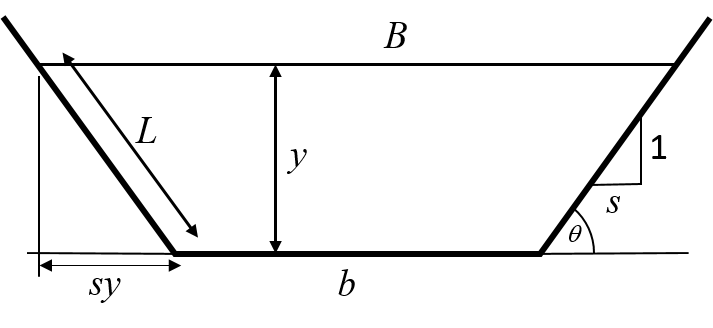
\includegraphics[width=8cm]{./images/section_trap_2018_a.png}
		\caption{A trapezoidal channel section}
		\label{fig:section_trap}
	\end{figure}
	For a trapezoidal channel with base $b$ and side slopes of $1$ vertical : $s$ horizontal, then we have:
	\begin{equation*}
	A = y(b+ys)
	\end{equation*}
	
	The wetted side slope, $L$ given by:
	\begin{align*}
	L &= \sqrt{y^2 + (ys)^2} \\
	&= y(1+s^2)^{1/2}
	\end{align*}
	Thus the wetted perimeter is
	\begin{align*}
	P &= b+ 2 L \\
	&= b + 2 y(1+s^2)^{1/2}
	\end{align*}
	Thus 
	\begin{equation*}
	R = \frac{y(b+ys)}{b+2y(1+s^2)^{1/2}}
	\end{equation*}
	
	And the top width
	\begin{equation*}
	B = b + 2ys
	\end{equation*}
	
	The Chezy equation, eqn \ref{eqn:chezy} for a trapezoidal channel becomes:
	\begin{equation}
	Q = C y_n(b+y_ns) \left( \frac{y_n(b+y_ns)}{b+2y_n(1+s^2)^{1/2}}\right)^{1/2}S_o^{1/2}
	\label{eqn:chezy_trap}
	\end{equation}
	
	The Manning equation, eqn \ref{eqn:manning} for a trapezoidal channel becomes:
	\begin{equation}
	Q = \frac{1}{n} \frac{[y_n(b+y_ns)]^{5/3}}{[b+2y_n(1+s^2)^{1/2}]^{2/3}} S_o^{1/2} \label{eqn:manning_trap}
	\end{equation}
	
	\subsubsection*{Circular Channels}
	\begin{figure}[H]
		\centering
		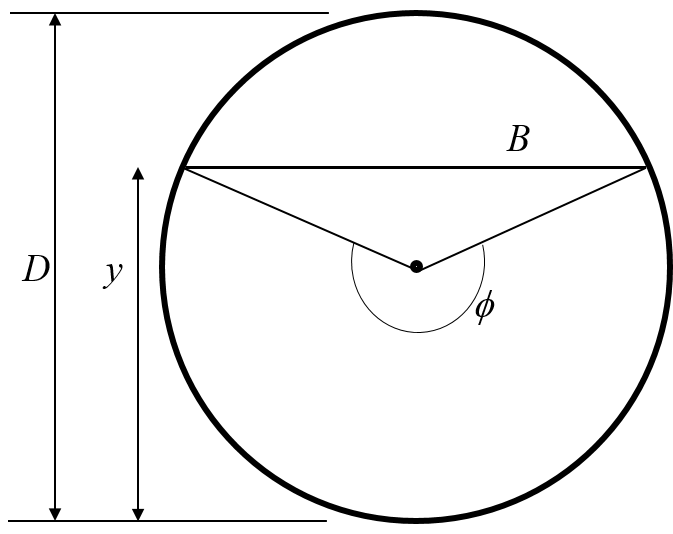
\includegraphics[width=7cm]{./images/section_circ.png}
		\caption{A circular channel section}
		\label{fig:section_circ}
	\end{figure}
	Circular channels a pipes that are not full (or \textit{just full} so at atmospheric presure).
	
	\[ 
	A = \frac{D^2}{8}(\phi - \sin \phi)
	\] 
	and 
	\[
	P = \frac{\phi D}{2}
	\]
	so
	\[
	R = \frac{A}{P} = \frac{D}{4}\left(1-\frac{\sin \phi}{\phi}\right)
	\]
	(Remember that in the above expressions $\phi$ is expressed in \textit{radians})
	
	The Chezy equation, eqn \ref{eqn:chezy} for channel of circular section becomes:
	\begin{align}
	Q &= C  \frac{D^2}{8}(\phi - \sin \phi)  \frac{D^{1/2}}{2}\left(1-\frac{\sin \phi}{\phi}\right)^{1/2} S_o^{1/2} \nonumber \\
	&= C  \frac{D^{5/2}}{16}(\phi - \sin \phi)  \left(1-\frac{\sin \phi}{\phi}\right)^{1/2} S_o^{1/2}
	\label{eqn:chezy_circ}
	\end{align}
	
	The Manning equation, eqn \ref{eqn:manning} for a channel of circular section  becomes:
	\begin{equation}
	Q = \frac{1}{n}  \frac{D^2}{8}(\phi - \sin \phi)
	\left[\frac{D}{4}\left(1-\frac{\sin \phi}{\phi}\right)\right]^{2/3} S_o^{1/2}
	\label{eqn:manning_circ}
	\end{equation}
	Which could be simplified in several ways, e.g.
	\begin{equation*}
	Q = \frac{1}{n}  \frac{D^{8/3}}{20.16}(\phi - \sin \phi)
	\left[\left(1-\frac{\sin \phi}{\phi}\right)\right]^{2/3} S_o^{1/2}
	\label{eqn:manning_circ2}
	\end{equation*}
	
	These equations are solved for $\phi$ and $y_n$ calculated from 
	\begin{equation*}
	y_n = \frac{D}{2} \left( 1 - \cos \frac{\phi}{2} \right)
	\end{equation*}
	
	
	
	\subsection*{Wide Rectangular Channels}
	For a \textit{wide} rectangular channel we can look at the equation for $R$ again. For a rectangular channel we have:
	\begin{equation*}
	R = \frac{By}{B+2y}
	\end{equation*}
	Dividing top and bottom by $B$ gives
	\begin{equation*}
	R = \frac{y}{1+\frac{2y}{B}}
	\end{equation*}
	As $B \to \infty$ then $\frac{2y}{B} \to 0$ therefore $R \to y$. \\
	So for a wide rectangular channel, when $B \gg y$, we can justifiably say:
	\begin{equation}
	R \approx y
	\end{equation}
	The Chezy equation, eqn \ref{eqn:chezy} for a wide channel becomes:
	\begin{align}
	Q &= By_{n} C y_{n}^{1/2} S_o^{1/2} \nonumber \\
	&= CBy_{n}^{3/2}S_o^{1/2}
	\label{eqn:chezy_wide}
	\end{align}
	
	The Manning equation, eqn \ref{eqn:manning} for a wide channel becomes:
	\begin{align}
	Q &= \frac{1}{n}By_{n} y_{n}^{1/6} y_{n}^{1/2} S_o^{1/2} \nonumber \\
	&= \frac{1}{n}By_{n}^{5/3}  S_o^{1/2}
	\label{eqn:manning_wide}
	\end{align}
	
	
	
	\subsubsection*{Unit Discharge}
	Sometime it is useful to quote flows in \textit{flow per unit width}. Which would be in the SI system flow per $m$.
	This is usually given the symbol of lower case $q$. It is thus defied:
	\begin{equation}
	\text{unit discharge } = q = \frac{Q}{B}
	\end{equation}
	
	The corresponding uniform floe equations are thus equation \ref{eqn:chezy_sq} or \ref{eqn:manning_sq} divided by top wide $B$:
	
	Chezy equation for unit discharge:
	\begin{equation}
	q = Cy^{3/2}S_o^{1/2}
	\label{eqn:chezy_unit}
	\end{equation}
	
	Manning equation for unit discharge:
	\begin{align}
	q = \frac{1}{n}y^{5/3}  S_o^{1/2}
	\label{eqn:manning_unit}
	\end{align}
	
	\subsubsection*{Normal depth in terms of Unit Discharge}
	An explicit equation for normal depth can be written from the Chezy equation \ref{eqn:chezy_unit}: 
	\begin{equation}
	y_{n} = \sqrt[3]{\frac{q^2}{C^2S_o}}
	\label{eqn:chezy_yn_unit_q}
	\end{equation}
	
	And similarly for normal depth can be written from the Manning's form \ref{eqn:manning_unit}: 
	\begin{equation}
	y_{n} = \left(\frac{qn}{S_o^{1/2}}\right)^{3/5}
	\label{eqn:manning_yn_unit_q}
	\end{equation}
	
	\subsubsection*{Fr and Critical depth in terms of Unit Discharge}
	While we are discussion unit discharge, it might be worth thinking about how the Froude number, Fr, would be defined in terms of $q$. Remembering the equation for Fr is $Fr = \frac{V}{\sqrt{gD_m}}$ and that $D_m = \frac{A}{B}$ then considering a rectangular channel and unit discharge:
	\begin{equation*}
	V = \frac{Q}{A}=\frac{Q}{by}=\frac{q}{y}
	\end{equation*}
	
	\begin{equation*}
	D_m = \frac{A}{B}=\frac{By}{B}=y
	\end{equation*}
	and
	\begin{equation}
	Fr  =\frac{q}{y} \frac{1}{g^{1/2}y^{1/2}}
	=\frac{q}{g^{1/2}y^{3/2}}
	\end{equation}
	
	And as \textit{critical depth}, $y_c$, is calculated by equating $Fr$ to 1, thus
	\begin{equation*}
	1 =\frac{q}{g^{1/2}y_{c}^{3/2}}
	\end{equation*}
	and
	\begin{equation*}
	y_{c}^{3/2} = \frac{q}{g^{1/2}}
	\end{equation*}
	\begin{equation}
	y_{c} = \sqrt[3]{\frac{q^2}{g}} = \left(\frac{q^2}{g}\right)^{1/3} 
	\end{equation}
	
	\subsection*{A note on the units of Chezy $C$ and  Manning $n$}
	
	Although the values of $C$ and $n$ are often quoted without unit they \textit{do} have units. 
	
	The units of $C$ are $m^{1/2}/s$, or $m^{1/2}s^{-1}$.
	
	The units of $n$ are $s / m^{1/3}$ or $s \; m^{-1/3}$.
	
	Unusually (but conveniently), though  $n$ has units, the value are always quoted in SI units but can be used in other systems of units. This is achieved by changing the Manning equation for that particular unit system. 
	
	Specifically for the system of \textit{English units} or \textit{imperial units} or, more commonly now, \textit{US customary units}, or even the $FPS$\footnote{Foot, Pound, Second} system,  where length is expressed in unit of $ft$ and discharge in $ft^3/s$, then  the Manning equation, eqn \ref{eqn:manning} is written: 
	\begin{align}
	Q = \frac{1.49}{n}AR^{2/3}S_o^{1/2}
	\label{eqn:manning_us}
	\end{align}
	where the $1.49$ is a factor that conveniently converts the units of the $n$ given in SI.\\
	(For reference, $(1 m)^{1/3}/s = (3.2808399 ft)^{1/3}/s = 1.4859 ft^{1/3}/s$ ).
	
	Having said that these are the units of $n$; they are indeed the units that balance the equation. However, if we look at the units physically we see that $n$, which is a \textit{roughness} measure, is a function of time. It is unlikely that, physically, in a steady state equation of flow, roughness changes with time. Some texts take this thought further and say that $n$ is in fact dimensionless and that the factor $1$ in SI and $1.49$ are in fact not pure numbers but dimensional constants, with units of  $m^{1/3} /s$, (or $ft^{1/3} /s$).

%\section{Second appendix}

\begin{thebibliography}{99}
\bibitem{chow59} Chow, VT, \emph{Open-Channel Hydraulics,} McGraw-Hill Book Co., 1959.
\bibitem{chadwick} Chadwick, A, and Morfett, J, \emph{Hydraulics in Civil and Environmental Engineering}, 2nd Ed, E \& FN Spon, 1993.
\bibitem{french94}	French, RH: Open-Channel Hydraulics, McGraw-Hill Book Co., 1994.
\end{thebibliography}
\end{document}